\documentclass[slidestop,compress,mathserif]{beamer}

%%% To get handouts:
%\documentclass[11pt,containsverbatim,handout]{beamer}
%% include when making handouts
%\usepackage{pgfpages}
%\pgfpagesuselayout{4 on 1}[letterpaper,landscape,border shrink=5mm]

%%% To get rid of solutions on handouts:
\newcommand{\soln}[1]{\textit{#1}}				% For slides
%\newcommand{\soln}[1]{ }	% For handouts

\usetheme{AnnArbor}

% Load color theme: There are a variety of color themes available, not limited to the ones listed below. Make sure to use only one at a time and comment out the rest.
%\usecolortheme{albatross}
%\usecolortheme{dolphin}
\usecolortheme{seahorse}
%\usecolortheme{seagull}

\usepackage{geometry}
\usepackage{graphicx}
\usepackage{amssymb}
%\usepackage{cancel}
\usepackage{epstopdf}
\usepackage{amsmath}  	% this permits text in eqnarray among other benefits
\usepackage{url}		% produces hyperlinks
\usepackage{hyperref}	% allows for color usage in tables
\usepackage[english]{babel}
\usepackage[latin1]{inputenc}
\usepackage{colortbl}	% allows for color usage in tables
\usepackage{multirow}	% allows for rows that span multiple rows in tables
\usepackage{color}		% this package has a variety of color options
\usepackage{pgf}
\usepackage{calc}
\usepackage{ulem}
\usepackage{multicol}
\usepackage{textcomp}
\usepackage{txfonts}
\usepackage{listings}
\usepackage{tikz}
\usepackage{array}
\usepackage{wasysym}
\usepackage{fancyvrb}


%%%%%%%%%%%%%%%%
% Remove navigation symbols
%%%%%%%%%%%%%%%%

\setbeamertemplate{navigation symbols}{}

%%%%%%%%%%%%%%%%
% User defined colors
%%%%%%%%%%%%%%%%

\xdefinecolor{oiB}{rgb}{0.22,0.52,0.72}
\definecolor{oiG}{rgb}{.298,.447,.114}
\xdefinecolor{hlblue}{rgb}{0.051,0.65,1}
\xdefinecolor{gray}{rgb}{0.5, 0.5, 0.5}
\xdefinecolor{darkGray}{rgb}{0.3, 0.3, 0.3}
\xdefinecolor{darkerGray}{rgb}{0.2, 0.2, 0.2}
\xdefinecolor{rubineRed}{rgb}{0.89,0,0.30}
\xdefinecolor{irishGreen}{rgb}{0,0.60,0}	
\definecolor{lightGreen}{rgb}{0.387,0.581,0.148} 

%%%%%%%%%%%%%%%%
% Template colors
%%%%%%%%%%%%%%%%

\setbeamercolor*{palette primary}{fg=white,bg= oiB!80!black!90}
\setbeamercolor*{palette secondary}{fg=black,bg= oiB!80!black}
\setbeamercolor*{palette tertiary}{fg=white,bg= oiB!80!black!80}
\setbeamercolor*{palette quaternary}{fg=white,bg= oiB}
\setbeamercolor{structure}{fg= oiB}
\setbeamercolor{frametitle}{bg= oiB!90}
\setbeamertemplate{blocks}[shadow=false]
\setbeamersize{text margin left=2em,text margin right=2em}

\setbeamercolor{code body}{bg=gray!20!white!80,fg=black}

%%%%%%%%%%%%%%%%
% Get rid of fancy enumerated list bullets
%%%%%%%%%%%%%%%%

\setbeamertemplate{enumerate items}[default]

%%%%%%%%%%%%%%%%
% Custom commands
%%%%%%%%%%%%%%%%

% degree
\newcommand{\degree}{\ensuremath{^\circ}}

% cite
\newcommand{\ct}[1]{
\vfill
{\tiny #1}}

% Note
\newcommand{\Note}[1]{
\rule{2.5cm}{0.25pt} \\ \textit{\footnotesize{\textcolor{rubineRed}{Note:} \textcolor{darkerGray}{#1}}}}

% Remember
\newcommand{\Remember}[1]{\textit{\scriptsize{\textcolor{orange}{Remember:} #1}}}

% expected counts
\newcommand{\ex}[1]{\textit{\textcolor{blue}{#1}}}

% red
\newcommand{\red}[1]{\textit{\textcolor{rubineRed}{#1}}}

% pink
\newcommand{\pink}[1]{\textit{\textcolor{rubineRed!90!white!50}{#1}}}

% green
\newcommand{\green}[1]{\textit{\textcolor{irishGreen}{#1}}}

% orange
\newcommand{\orange}[1]{\textit{\textcolor{orange}{#1}}}

% links: webURL, webLin, appLink
\newcommand{\webURL}[1]{\urlstyle{same}{ \textit{\textcolor{darkGray}{\url{#1}}}}}
\newcommand{\webLink}[2]{\href{#1}{\textcolor{darkGray}{{#2}}}}
\newcommand{\appLink}[2]{\href{#1}{\textcolor{white}{{#2}}}}

% mail
\newcommand{\mail}[1]{\href{mailto:#1}{\textit{\textcolor{darkGray}{#1}}}}

% highlighting: hl, hlGr, mathhl
\newcommand{\hl}[1]{\textit{\textcolor{hlblue}{#1}}}
\newcommand{\hlGr}[1]{\textit{\textcolor{lightGreen}{#1}}}
\newcommand{\mathhl}[1]{\textcolor{hlblue}{\ensuremath{#1}}}

% two col: two columns
\newenvironment{twocol}[4]{
\begin{columns}[c]
\column{#1\textwidth}
#3
\column{#2\textwidth}
#4
\end{columns}
}

% slot (for probability calculations)
\newenvironment{slot}[2]{
\begin{array}{c} 
\underline{#1} \\ 
#2
\end{array}
}

% pr: left and right parentheses
\newcommand{\pr}[1]{
\left( #1 \right)
}

% solnMult: solutions for practice questions

\newcommand{\solnMult}[1]{
\item[] \vspace{-0.59cm}
\only<1>{\item #1}
\soln{\only<2->{\item \red{#1}}}
}

% cancel
\newcommand{\cancel}[1]{%
    \tikz[baseline=(tocancel.base)]{
        \node[inner sep=0pt,outer sep=0pt] (tocancel) {#1};
        \draw[red, line width=0.5mm] (tocancel.south west) -- (tocancel.north east);
    }%
}

% removepagenumbers
\newcommand{\removepagenumbers}{% 
  \setbeamertemplate{footline}{
    %
    \begin{beamercolorbox}[colsep=1.5pt]{upper separation line foot}
    \end{beamercolorbox}
    \begin{beamercolorbox}[ht=2.5ex,dp=1.125ex,%
      leftskip=.3cm,rightskip=.3cm plus1fil]{author in head/foot}%
      \leavevmode{\usebeamerfont{author in head/foot}\insertshortauthor}%
%      \hfill%
%      {\usebeamerfont{author in head/foot}\usebeamercolor[fg]{institute in head/foot}\insertshortinstitute}%
    \end{beamercolorbox}%
    \begin{beamercolorbox}[ht=2.5ex,dp=1.125ex,%
      leftskip=.3cm,rightskip=.3cm plus1fil]{title in head/foot}%
      {\usebeamerfont{title in head/foot}\insertshorttitle}%
      \hfill%
      {\usebeamerfont{author in head/foot}\usebeamercolor[fg]{institute in head/foot}\insertshortinstitute}%
    \end{beamercolorbox}%
    \begin{beamercolorbox}[colsep=1.5pt]{lower separation line foot}
    \end{beamercolorbox}
    }
}

%%%%%%%%%%%%%%%%
% Custom boxes
%%%%%%%%%%%%%%%%

% app: application exercise

\setbeamercolor{app body}{bg=white,fg=oiG}

\newcommand{\app}[1]{
\begin{beamerboxesrounded}[shadow = false, lower = app body]{}
#1
\end{beamerboxesrounded}
}

% dq: discussion question

\setbeamercolor{disc ques body}{bg=white,fg=oiB}

\newcommand{\dq}[1]{
\begin{beamerboxesrounded}[shadow = false, lower = disc ques body]{}
#1
\end{beamerboxesrounded}
}

% pq: practice question

\setbeamercolor{prac ques body}{bg=white,fg=oiB}

\newcommand{\pq}[1]{
\begin{beamerboxesrounded}[shadow = false, lower = prac ques body]{}
#1
\end{beamerboxesrounded}
}

% formula

\setbeamercolor{formula body}{bg=white,fg=oiB!55!black!95}

\newcommand{\formula}[1]{
\begin{beamerboxesrounded}[shadow = false, lower = formula body]{}
#1
\end{beamerboxesrounded}
}


%%%%%%%%%%%%%%%%
% Change margin
%%%%%%%%%%%%%%%%

\newenvironment{changemargin}[2]{%
\begin{list}{}{%
\setlength{\topsep}{0pt}%
\setlength{\leftmargin}{#1}%
\setlength{\rightmargin}{#2}%
\setlength{\listparindent}{\parindent}%
\setlength{\itemindent}{\parindent}%
\setlength{\parsep}{\parskip}%
}%
\item}{\end{list}}

%%%%%%%%%%%%%%%%
% Footnote
%%%%%%%%%%%%%%%%

\long\def\symbolfootnote[#1]#2{\begingroup%
\def\thefootnote{\fnsymbol{footnote}}\footnote[#1]{#2}\endgroup}

%%%%%%%%%%%%%%%%
% Commands from the book
%%%%%%%%%%%%%%%%

\newenvironment{data}[1]{\texttt{#1}}{}
\newenvironment{var}[1]{\texttt{#1}}{}
\newenvironment{resp}[1]{\texttt{#1}}{}

%%%%%%%%%%%%%%%%
% Graphics
%%%%%%%%%%%%%%%%

\DeclareGraphicsRule{.tif}{png}{.png}{`convert #1 `dirname #1`/`basename #1 .tif`.png}

%%%%%%%%%%%%%%%%
% TOC slides
%%%%%%%%%%%%%%%%

\AtBeginSection[] 
{ 
  \addtocounter{framenumber}{-1} 
  % 
  {\removepagenumbers 
    \begin{frame}<beamer> [shrink]
    \tableofcontents[currentsection,hideothersubsections] 
    \vspace{0.25cm}
  \end{frame} 
  } 
} 

%%%%%%%%%%%%%%%%%%%%%

\title[Chp 1: Intro. to data]{Chapter 1: Introduction to data}
\author{OpenIntro Statistics, 2nd Edition}
\date{}
\institute{}

%%%%%%%%%%%%%%%%%%%%%

\begin{document}

%%%%%%%%%%%%%%%%%%%%%

% Title Page

\begin{frame}[plain]

\titlepage

\end{frame}

%%%%%%%%%%%%%%%%%%%%%%%%%%%%%%%%%%%%

\section{Case study}

%%%%%%%%%%%%%%%%%%%%%%%%%%%%%%%%%%%%

\begin{frame}
\frametitle{Treating Chronic Fatigue Syndrome}

\begin{itemize}

\item Objective: Evaluate the effectiveness of cognitive-behavior therapy for chronic fatigue syndrome.

\item Participant pool: 142 patients who were recruited from referrals by primary care physicians and consultants to a hospital clinic specializing in chronic fatigue syndrome.

\item Actual participants: Only 60 of the 142 referred patients entered the study. Some were excluded because they didn't meet the diagnostic criteria, some had other health issues, and some refused to be a part of the study.

\end{itemize}

\ct{Deale et. al. \textit{Cognitive behavior therapy for chronic fatigue syndrome: A randomized controlled trial}. The American Journal of Psychiatry 154.3 (1997).}

\end{frame}

%%%%%%%%%%%%%%%%%%%%%%%%%%%%%%%%%%%%

\begin{frame}
\frametitle{Study design}

\begin{itemize}

\item Patients randomly assigned to treatment and control groups, 30 patients in each group:
\begin{itemize}
\item \hl{Treatment}: Cognitive behavior therapy -- collaborative, educative, and with a behavioral emphasis. Patients were shown on how activity could be increased steadily and safely without exacerbating symptoms.
\item \hl{Control:} Relaxation -- No advice was given about how activity could be increased. Instead progressive muscle relaxation, visualization, and rapid relaxation skills were taught.
\end{itemize}

\end{itemize}

\end{frame}

%%%%%%%%%%%%%%%%%%%%%%%%%%%%%%%%%%%%

\begin{frame}
\frametitle{Results}

The table below shows the distribution of patients with good outcomes at 6-month follow-up. Note that 7 patients dropped out of the study: 3 from the treatment and 4 from the control group.

\begin{center}
\begin{tabular}{ll  cc c} 
			&				& \multicolumn{2}{c}{\textit{Good outcome}} \\
\cline{3-4}
			&							& Yes 	& No 	& Total	\\
\cline{2-5}
							&Treatment 	& 19	 	& 8		& 27 	\\
\raisebox{1.5ex}[0pt]{\textit{Group}}	&Control		& 5	 	& 21	 	& 26 \\
\cline{2-5}
							&Total		& 24		& 29		& 53
\end{tabular}
\end{center}

\pause

\begin{itemize}

\item Proportion with good outcomes in treatment group:
\[ 19 / 27 \approx 0.70 \rightarrow 70\% \]

\pause

\item Proportion with good outcomes in control group:
\[ 5 / 26 \approx 0.19 \rightarrow 19\% \]

\end{itemize}

\end{frame}

%%%%%%%%%%%%%%%%%%%%%%%%%%%%%%%%%%%%

\begin{frame}
\frametitle{Understanding the results}

\dq{Do the data show a ``real" difference between the groups?}

\pause

\begin{itemize}

\item Suppose you flip a coin 100 times. While the chance a coin lands heads in any given coin flip is 50\%, we probably won't observe exactly 50 heads. This type of fluctuation is part of almost any type of data generating process.

\item The observed difference between the two groups (70 - 19 = 51\%) may be real, or may be due to natural variation.

\item Since the difference is quite large, it is more believable that the difference is real.

\item We need statistical tools to determine if the difference is so large that we should reject the notion that it was due to chance.

\end{itemize}

\end{frame}

%%%%%%%%%%%%%%%%%%%%%%%%%%%%%%%%%%%%

\begin{frame}
\frametitle{Generalizing the results}

\dq{Are the results of this study generalizable to all patients with chronic fatigue syndrome?}

\pause

These patients had specific characteristics and volunteered to be a part of this study, therefore they may not be representative of all patients with chronic fatigue syndrome. While we cannot immediately generalize the results to all patients, this first study is encouraging. The method works for patients with some narrow set of characteristics, and that gives hope that it will work, at least to some degree, with other patients.


\end{frame}

%%%%%%%%%%%%%%%%%%%%%%%%%%%%%%%%%%%%

%%%%%%%%%%%%%%%%%%%%%%%%%%%%%%%%%%%%

\section{Data basics}

%%%%%%%%%%%%%%%%%%%%%%%%%%%%%%%%%%%%

\subsection{Observations and variables}

\begin{frame}
\frametitle{Data matrix}

Data collected on students in a statistics class on a variety of variables:

\begin{center}
\begin{tabular}{l cccc l}
		& \hl{variable} \\
		& \hl{$\downarrow$}	 \\
\cline{1-5}
Stu.	&	\var{gender}	&	\var{intro\_extra} & $\cdots$ & \var{dread} \\
\cline{1-5}
1 & male & extravert  & $\cdots$ & 3 \\ 
  2 & female & extravert & $\cdots$ & 2 \\ 
  3 & female & introvert  & $\cdots$ & 4 & \hl{$\leftarrow$}  \\ 
  4 & female & extravert  & $\cdots$ & 2 & \hl{observation} \\
$\vdots$	&	$\vdots$	  &	$\vdots$  &	$\vdots$ &	$\vdots$ \\
86	& male & extravert & $\cdots$& 3 \\
\cline{1-5}
\end{tabular}
\end{center}

\end{frame}

%%%%%%%%%%%%%%%%%%%%%%%%%%%%%%%%%%%%

\subsection{Types of variables}

\begin{frame}
\frametitle{Types of variables}

\begin{center}
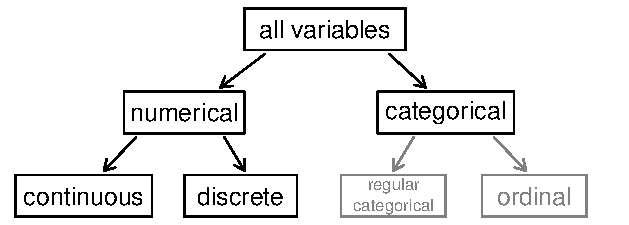
\includegraphics[width=0.9\textwidth]{1-2_data_basics/figures/variables/variables}
\end{center}

\end{frame}

%%%%%%%%%%%%%%%%%%%%%%%%%%%%%%%%%%%

\begin{frame}
\frametitle{Types of variables (cont.)}

\begin{center}
{\footnotesize
\begin{tabular}{c ccc cc}
  \hline
 & \var{gender} & \var{sleep} & \var{bedtime} & \var{countries} & \var{dread} \\
  \hline
1 & male & 5 & 12-2 & 13 & 3 \\ 
  2 & female & 7 & 10-12 & 7 & 2 \\ 
  3 & female & 5.5 & 12-2 & 1 & 4 \\ 
  4 & female & 7 & 12-2 &  & 2 \\ 
  5 & female & 3 & 12-2 & 1 & 3 \\ 
  6 & female & 3 & 12-2 & 9 & 4 \\ 
  \hline
\end{tabular}
}
\end{center}

\begin{itemize}
\item \var{gender}: \pause \soln{\only<2->{categorical}} \pause
\item \var{sleep}: \pause \soln{\only<4->{numerical, continuous}} \pause
\item \var{bedtime}: \pause \soln{\only<6->{categorical, ordinal}} \pause
\item \var{countries}: \pause \soln{\only<8->{numerical, discrete}} \pause
\item \var{dread}: \pause \soln{\only<10->{categorical, ordinal - could also be used as numerical}}
\end{itemize}

\end{frame}

%%%%%%%%%%%%%%%%%%%%%%%%%%%%%%%%%%%

\begin{frame}
\frametitle{Practice}

\pq{What type of variable is a telephone area code?}

\begin{enumerate}[(a)]
\item numerical, continuous
\item numerical, discrete
\solnMult{categorical}
\item categorical, ordinal
\end{enumerate}

\end{frame}

%%%%%%%%%%%%%%%%%%%%%%%%%%%%%%%%%%%

\subsection{Relationships among variables}

%%%%%%%%%%%%%%%%%%%%%%%%%%%%%%%%%%%

\begin{frame}
\frametitle{Relationships among variables}

\dq{Does there appear to be a relationship between number of alcoholic drinks consumed per week and age at first alcohol consumption?}

\begin{center}
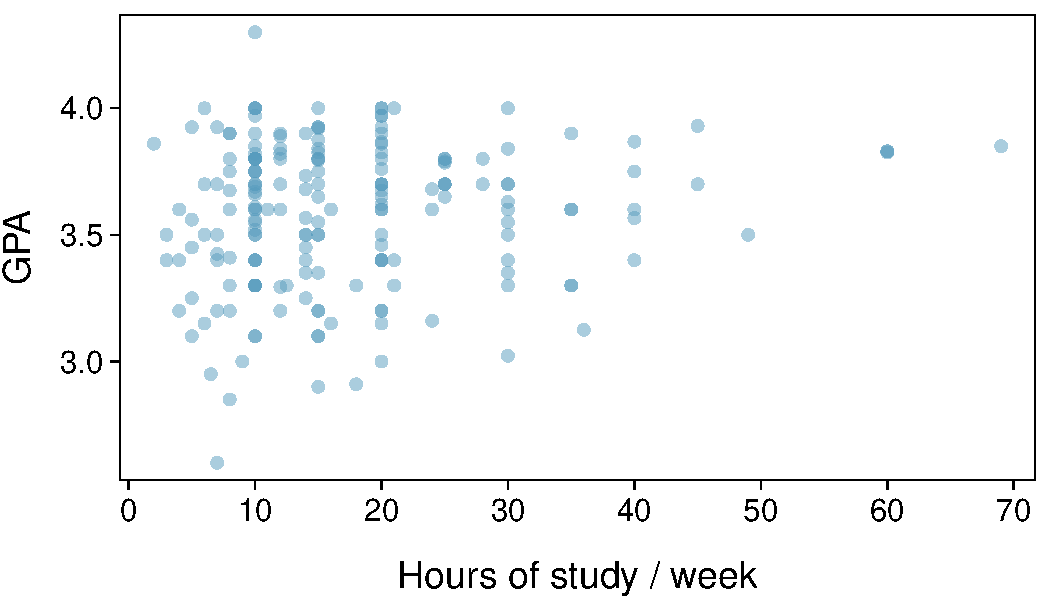
\includegraphics[width=0.7\textwidth]{1-2_data_basics/figures/gpa_study_hours/gpa_study_hours}
\end{center}

\pause

\dq{Can you spot anything unusual about any of the data points?}

\soln{\pause{There is one student with GPA $>$ 4.0, this is likely a data error.}}

\end{frame}

%%%%%%%%%%%%%%%%%%%%%%%%%%%%%%%%%%%

\subsection{Associated and independent variables}

%%%%%%%%%%%%%%%%%%%%%%%%%%%%%%%%%%%

\begin{frame}
\frametitle{Practice}

\twocol{0.5}{0.5}
{
\pq{Based on the scatterplot on the right, which of the following statements is correct about the head and skull lengths of possums?}
}
{
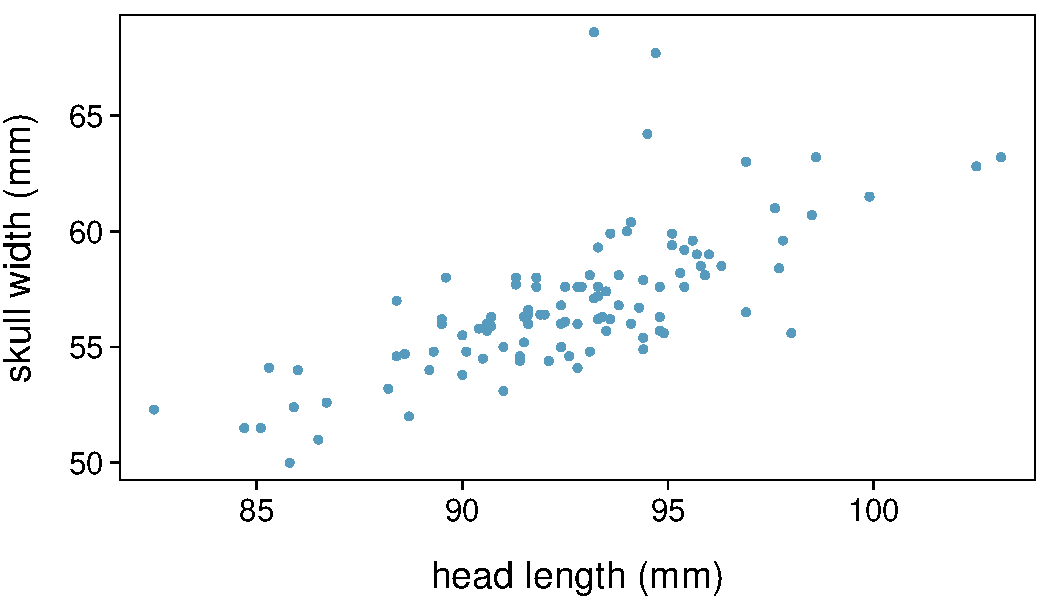
\includegraphics[width=\textwidth]{1-2_data_basics/figures/possum_head_skull/possum_head_skull}
}

\begin{enumerate}[(a)]
\item There is no relationship between head length and skull width, i.e. the variables are independent.
\solnMult{Head length and skull width are positively associated.}
\item Skull width and head length are negatively associated.
\item A longer head causes the skull to be wider.
\item A wider skull causes the head to be longer.
\end{enumerate}

\end{frame}

%%%%%%%%%%%%%%%%%%%%%%%%%%%%%%%%%%%

\begin{frame}
\frametitle{Associated vs. independent}

\begin{itemize}

\item When two variables show some connection with one another, they are called \hl{associated} variables.
\begin{itemize}
\item Associated variables can also be called \hl{dependent} variables and vice-versa.
\end{itemize}

\item If two variables are not associated, i.e. there is no evident connection between the two, then they are said to be \hl{independent}.

\end{itemize}

\end{frame}

%%%%%%%%%%%%%%%%%%%%%%%%%%%%%%%%%%%%
%%%%%%%%%%%%%%%%%%%%%%%%%%%%%%%%%%%%

\section{Overview of data collection principles}

%%%%%%%%%%%%%%%%%%%%%%%%%%%%%%%%%%%%

\subsection{Populations and samples}

%%%%%%%%%%%%%%%%%%%%%%%%%%%%%%%%%%%%

\begin{frame}
\frametitle{Populations and samples}

\twocol{0.5}{0.5}{
\begin{center}
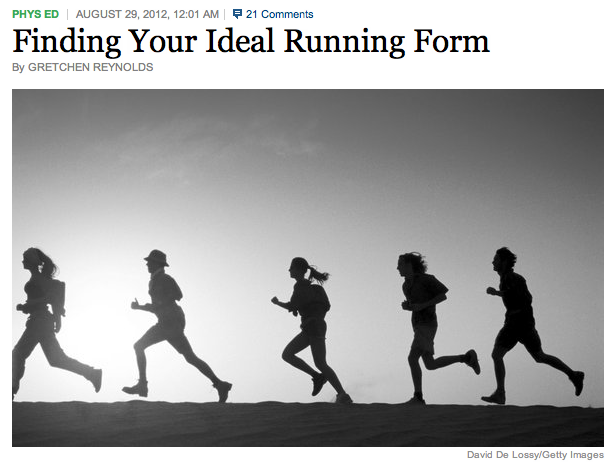
\includegraphics[width=\textwidth]{1-3_data_collection_principles/figures/running}
\end{center}
\vspace{-0.5cm}
{\tiny \webURL{http://well.blogs.nytimes.com/2012/08/29/finding-your-ideal-running-form}}
}
{
\hl{Research question:} Can people become better, more efficient runners on their own, merely by running? \\

\pause 

\hl{Population of interest:} \soln{\pause All people}
}
\pause 
$\:$ \\
\hl{Sample:} Group of adult women who recently joined a running group

\pause

\hl{Population to which results can be generalized:} \soln{\pause Adult women, if the data are randomly sampled}

\end{frame}

%%%%%%%%%%%%%%%%%%%%%%%%%%%%%%%%%%%%

\subsection{Anecdotal evidence}

%%%%%%%%%%%%%%%%%%%%%%%%%%%%%%%%%%%%

\begin{frame}
\frametitle{Anecdotal evidence and early smoking research}

\begin{itemize}

\item Anti-smoking research started in the 1930s and 1940s when cigarette smoking became increasingly popular. While some smokers seemed to be sensitive to cigarette smoke, others were completely unaffected.

\item Anti-smoking research was faced with resistance based on \hl{anecdotal evidence} such as ``My uncle smokes three packs a day and he's in perfectly good health", evidence based on a limited sample size that might not be representative of the population.

\item It was concluded that ``smoking is a complex human behavior, by its nature difficult to study, confounded by human variability."

\item In time researchers were able to examine larger samples of cases (smokers), and trends showing that smoking has negative health impacts became much clearer.

\end{itemize}

\ct{Brandt, \textit{The Cigarette Century} (2009), Basic Books.}

\end{frame}

%%%%%%%%%%%%%%%%%%%%%%%%%%%%%%%%%%%%

\subsection{Sampling from a population}

\begin{frame}
\frametitle{Census}

\begin{itemize}

\item Wouldn't it be better to just include everyone and ``sample" the entire population? 

\begin{itemize}
\item This is called a \hl{census}.
\end{itemize}

\pause

\item There are problems with taking a census:

\begin{itemize}
\item It can be difficult to complete a census: there always seem to be some individuals who are hard to locate or hard to measure. \textit{And these difficult-to-find people may have certain characteristics that distinguish them from the rest of the population.}
\item Populations rarely stand still. Even if you could take a census, the population changes constantly, so it's never possible to get a perfect measure.
\item Taking a census may be more complex than sampling.
\end{itemize}

\end{itemize}

\end{frame}

%%%%%%%%%%%%%%%%%%%%%%%%%%%%%%%%%%%%%

\begin{frame}

\vfill

\begin{center}
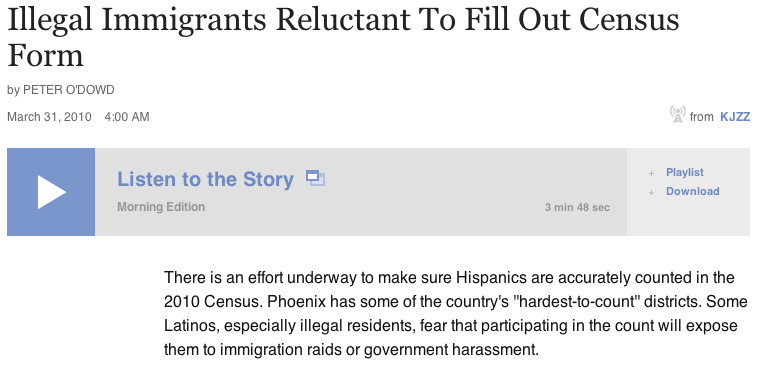
\includegraphics[width=0.90\textwidth]{1-3_data_collection_principles/figures/census_illegal_immig}
\end{center}

\ct{\webURL{http://www.npr.org/templates/story/story.php?storyId=125380052}}

\end{frame}

%%%%%%%%%%%%%%%%%%%%%%%%%%%%%%%%%%%%%

\begin{frame}
\frametitle{Exploratory analysis to inference}

\begin{itemize}

\item Sampling is natural.

\pause

\item Think about sampling something you are cooking - you taste (examine) a small part of what you're cooking to get an idea about the dish as a whole.

\pause

\item When you taste a spoonful of soup and decide the spoonful you tasted isn't salty enough, that's \hl{exploratory analysis}.

\pause

\item If you generalize and conclude that your entire soup needs salt, that's an \hl{inference}.

\pause

\item For your inference to be valid, the spoonful you tasted (the sample) needs to be \hl{representative} of the entire pot (the population).

\begin{itemize}
\item If your spoonful comes only from the surface and the salt is collected at the bottom of the pot, what you tasted is probably not representative of the whole pot.
\item If you first stir the soup thoroughly before you taste, your spoonful will more likely be representative of the whole pot.
\end{itemize}

\end{itemize}

\end{frame}

%%%%%%%%%%%%%%%%%%%%%%%%%%%%%%%%%%%%

\begin{frame}
\frametitle{Sampling bias}

\begin{itemize}

\item \hl{Non-response:} If only a small fraction of the randomly sampled people choose to respond to a survey, the sample may no longer be representative of the population.

\pause

\item \hl{Voluntary response:} Occurs when the sample consists of people who volunteer to respond because they have strong opinions on the issue. Such a sample will also not be representative of the population.

\pause

\begin{center}
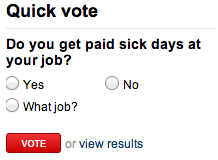
\includegraphics[width=0.25\textwidth]{1-3_data_collection_principles/figures/vol_resp_bias/vol_resp_bias_q}\pause
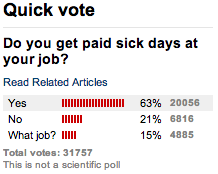
\includegraphics[width=0.25\textwidth]{1-3_data_collection_principles/figures/vol_resp_bias/vol_resp_bias_res} \\
{\tiny cnn.com, Jan 14, 2012}
\end{center}

\pause

\item \hl{Convenience sample:} Individuals who are easily accessible are more likely to be included in the sample.

\end{itemize}

\end{frame}

%%%%%%%%%%%%%%%%%%%%%%%%%%%%%%%%%%%%

\begin{frame}
\frametitle{Sampling bias example: Landon vs. FDR}

A historical example of a biased sample yielding misleading results: \\

$\:$ \\

\begin{columns}[c]

\column{0.35\textwidth}

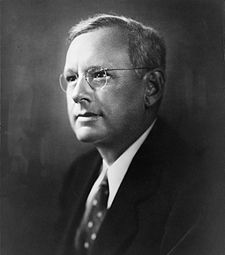
\includegraphics[width= \textwidth]{1-3_data_collection_principles/figures/landon_fdr/landon}

\column{0.3\textwidth}
In 1936, Landon sought the Republican presidential nomination opposing the re-election of FDR.

\column{0.35\textwidth}

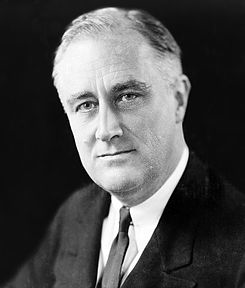
\includegraphics[width= \textwidth]{1-3_data_collection_principles/figures/landon_fdr/fdr}

\end{columns}

\end{frame}

%%%%%%%%%%%%%%%%%%%%%%%%%%%%%%%%%%%%%

\begin{frame}
\frametitle{The Literary Digest Poll}

\begin{columns}

\column{0.7\textwidth}

\begin{itemize}

\item The Literary Digest polled about 10 million Americans, and got responses from about 2.4 million.

\item The poll showed that Landon would likely be the overwhelming winner and FDR would get only 43\% of the votes.

\item Election result:  FDR won, with 62\% of the votes.

\end{itemize}

\column{0.3\textwidth}


\includegraphics[width= \textwidth]{1-3_data_collection_principles/figures/literaryDigest}

\end{columns}

\begin{itemize}

\item The magazine was completely discredited because of the poll, and was soon discontinued.

\end{itemize}

\end{frame}

%%%%%%%%%%%%%%%%%%%%%%%%%%%%%%%%%%%%%

\begin{frame}
\frametitle{The Literary Digest Poll -- what went wrong?}

\begin{itemize}

\item The magazine had surveyed

\begin{itemize}

\item its own readers,

\item registered automobile owners, and

\item registered telephone users.

\end{itemize}

\item These groups had incomes well above the national average of the day (remember, this is Great Depression era) which resulted in lists of voters far more likely to support Republicans than a truly \hl{typical} voter of the time, i.e. the sample was not representative of the American population at the time.

\end{itemize}

\end{frame}

%%%%%%%%%%%%%%%%%%%%%%%%%%%%%%%%%%%%%

\begin{frame}
\frametitle{Large samples are preferable, but...}

\begin{itemize}

\item The Literary Digest election poll was based on a sample size of 2.4 million, which is huge, but since the sample was \hl{biased}, the sample did not yield an accurate prediction.

\item Back to the soup analogy: If the soup is not well stirred, it doesn't matter how large a spoon you have, it will still not taste right. If the soup is well stirred, a small spoon will suffice to test the soup.

\end{itemize}

\end{frame}

%%%%%%%%%%%%%%%%%%%%%%%%%%%%%%%%%%%%%

\begin{frame}[shrink]
\frametitle{Practice}

{\small
\pq{A school district is considering whether it will no longer allow high school students to park at school after two recent accidents where students were severely injured. As a first step, they survey parents by mail, asking them whether or not the parents would object to this policy change. Of 6,000 surveys that go out, 1,200 are returned. Of these 1,200 surveys that were completed, 960 agreed with the policy change and 240 disagreed. Which of the following statements are true?}

\begin{enumerate}[I.]
\item Some of the mailings may have never reached the parents.
\item The school district has strong support from parents to move forward with the policy approval.
\item It is possible that majority of the parents of high school students disagree with the policy change.
\item The survey results are unlikely to be biased because all parents were mailed a survey. 
\end{enumerate}

\begin{multicols}{5}
\begin{enumerate}[(a)]
\item Only I
\item I and II
\solnMult{I and III}
\item III and IV
\item Only IV
\end{enumerate}
\end{multicols}
}

\end{frame}

%%%%%%%%%%%%%%%%%%%%%%%%%%%%%%%%%%%%%

\subsection{Explanatory and response variables}

%%%%%%%%%%%%%%%%%%%%%%%%%%%%%%%%%%%%%

\begin{frame}
\frametitle{Explanatory and response variables}

\begin{itemize}

\item To identify the explanatory variable in a pair of variables, identify which of the two is suspected of affecting the other:

\begin{center}
explanatory variable $\xrightarrow{might~affect}$response variable
\end{center}

\item Labeling variables as explanatory and response does not guarantee the relationship between the two is actually causal, even if there is an association identified between the two variables. We use these labels only to keep track of which variable we suspect affects the other.

\end{itemize}

\end{frame}

%%%%%%%%%%%%%%%%%%%%%%%%%%%%%%%%%%%%%

\subsection{Observational studies and experiments}

%%%%%%%%%%%%%%%%%%%%%%%%%%%%%%%%%%%%%

\begin{frame}
\frametitle{Observational studies and experiments}

\begin{itemize}

\item \hl{Observational study:} Researchers collect data in a way that does not directly interfere with how the data arise, i.e. they merely ``observe", and can only establish an association between the explanatory and response variables.

\pause

\item \hl{Experiment:} Researchers randomly assign subjects to various treatments in order to establish causal connections between the explanatory and response variables.

\pause

\item If you're going to walk away with one thing from this class, let it be ``correlation does not imply causation".

\begin{center}
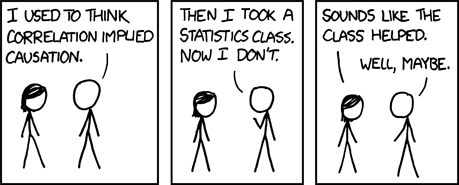
\includegraphics[width=0.55\textwidth]{1-3_data_collection_principles/figures/xkcd_correlation} \\
{\tiny \webURL{http://xkcd.com/552/}}
\end{center}

\end{itemize}

\end{frame}

%%%%%%%%%%%%%%%%%%%%%%%%%%%%%%%%%%%%%
%%%%%%%%%%%%%%%%%%%%%%%%%%%%%%%%%%%%%

\section{Observational studies and sampling strategies}

%%%%%%%%%%%%%%%%%%%%%%%%%%%%%%%%%%%%

\subsection{Confounding}

%%%%%%%%%%%%%%%%%%%%%%%%%%%%%%%%%%%%

\begin{frame}
\frametitle{}

\begin{center}
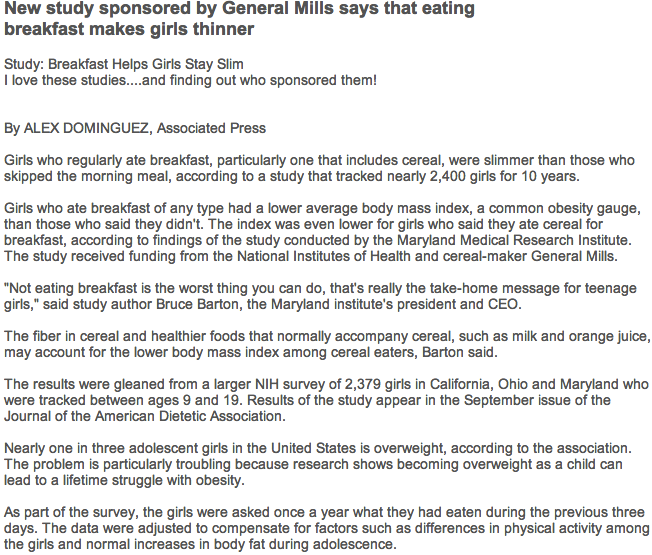
\includegraphics[width=0.80\textwidth]{1-4_obs_studies_sampling/figures/breakfast/breakfast1}
\end{center}

{\tiny \webURL{http://www.peertrainer.com/LoungeCommunityThread.aspx?ForumID=1\&ThreadID=3118}}

\end{frame}

%%%%%%%%%%%%%%%%%%%%%%%%%%%%%%%%%%%%

\begin{frame}
\frametitle{}

\dq{What type of study is this, observational study or an experiment?
{\footnotesize \textit{``Girls who regularly ate breakfast, particularly one that includes cereal, were slimmer than those who skipped the morning meal, according to a study that tracked nearly 2,400 girls for 10 years. [...] As part of the survey, the girls were asked once a year what they had eaten during the previous three days."}}
}

\soln{\onslide<2->{This is an \hl{observational study} since the researchers merely observed the behavior of the girls (subjects) as opposed to imposing treatments on them.}}

\dq{What is the conclusion of the study?}

\soln{\onslide<3->{There is an \hl{association} between girls eating breakfast and being slimmer.}}

\dq{Who sponsored the study?}

\soln{\onslide<4->{General Mills.}}

\end{frame}

%%%%%%%%%%%%%%%%%%%%%%%%%%%%%%%%%%%%

\begin{frame}[shrink]
\frametitle{3 possible explanations}

\pause

\begin{enumerate}

\item Eating breakfast causes girls to be thinner.
\begin{center}

\includegraphics[width=0.5\textwidth]{1-4_obs_studies_sampling/figures/breakfast/breakfast2}
\end{center}

\pause

\item Being thin causes girls to eat breakfast.
\begin{center}

\includegraphics[width=0.5\textwidth]{1-4_obs_studies_sampling/figures/breakfast/breakfast3}
\end{center}

\pause

\item A third variable is responsible for both. What could it be? \\
An extraneous variable that affects both the explanatory and the response variable and that make it seem like there is a relationship between the two are called \hl{confounding} variables.
\begin{center}
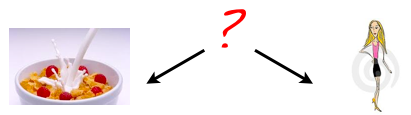
\includegraphics[width=0.5\textwidth]{1-4_obs_studies_sampling/figures/breakfast/breakfast4}
\end{center}

\end{enumerate}


{\tiny Images from: \webURL{http://www.appforhealth.com/wp-content/uploads/2011/08/ipn-cerealfrijo-300x135.jpg},  \webURL{http://www.dreamstime.com/stock-photography-too-thin-woman-anorexia-model-image2814892}.}



\end{frame}

%%%%%%%%%%%%%%%%%%%%%%%%%%%%%%%%%%%%

\begin{frame}
\frametitle{Prospective vs. retrospective studies}

\begin{itemize}

\item A \hl{prospective} study identifies individuals and collects information as events unfold. 
\begin{itemize}
\item Example: The Nurses Health Study has been recruiting registered nurses and then collecting data from them using questionnaires since 1976.
\end{itemize}

\item \hl{Retrospective studies} collect data after events have taken place.
\begin{itemize}
\item Example: Researchers reviewing past events in medical records.
\end{itemize}

\end{itemize}

\end{frame}

%%%%%%%%%%%%%%%%%%%%%%%%%%%%%%%%%%%

\subsection{Sampling strategies}

%%%%%%%%%%%%%%%%%%%%%%%%%%%%%%%%%%%

\begin{frame}
\frametitle{Obtaining good samples}

\begin{itemize}

\item Almost all statistical methods are based on the notion of implied randomness. 

\item If observational data are not collected in a random framework from a population, these statistical methods -- the estimates and errors associated with the estimates -- are not reliable.

\item Most commonly used random sampling techniques are \hl{simple}, \hl{stratified}, and \hl{cluster} sampling.

\end{itemize}

\end{frame}

%%%%%%%%%%%%%%%%%%%%%%%%%%%%%%%%%%%%

\begin{frame}
\frametitle{Simple random sample}

Randomly select cases from the population, where there is no implied connection between the points that are selected.

\begin{center}
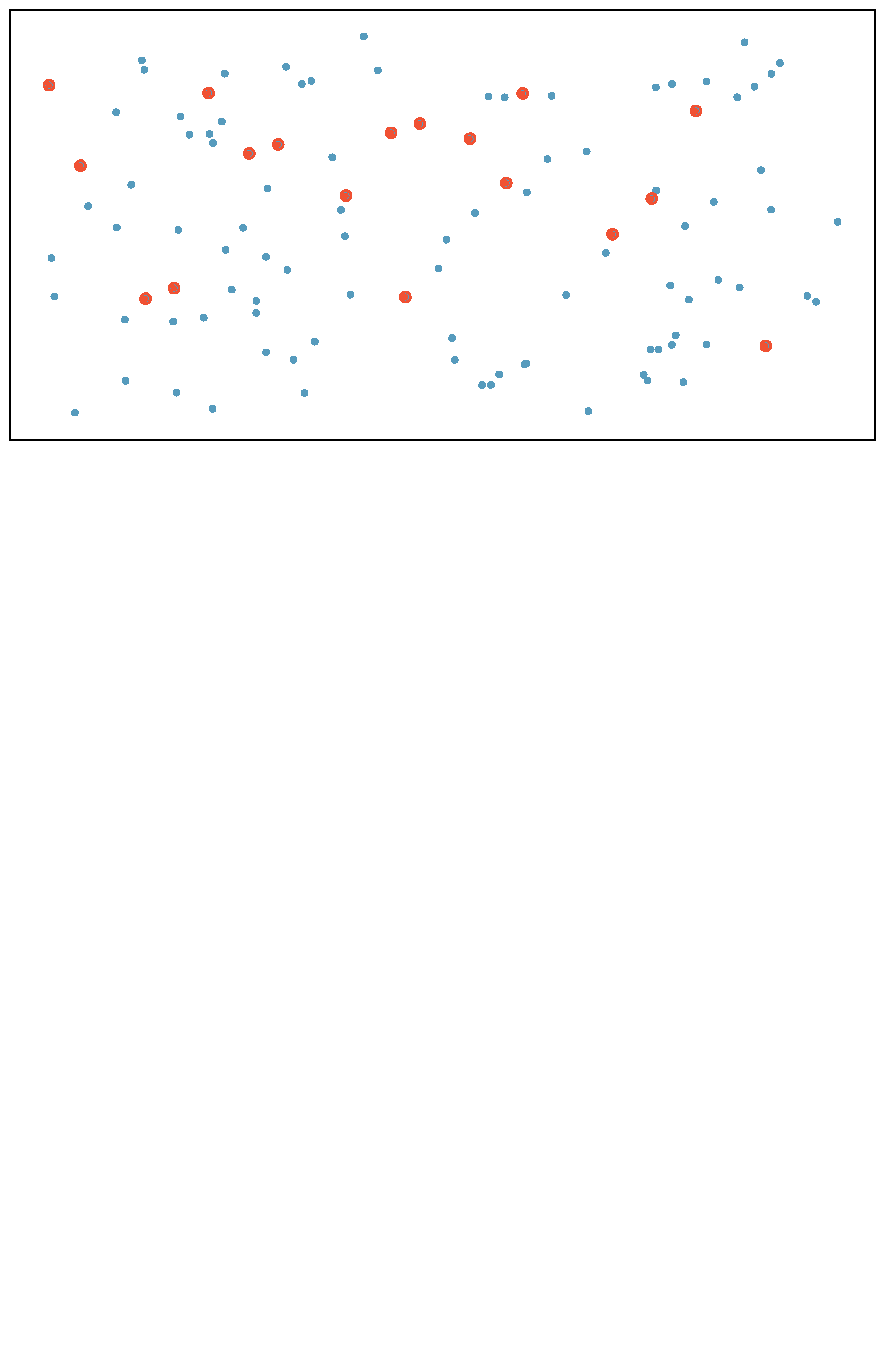
\includegraphics[width=0.9\textwidth]{1-4_obs_studies_sampling/figures/sampling_methods/srs}
\end{center}

\end{frame}

%%%%%%%%%%%%%%%%%%%%%%%%%%%%%%%%%%%%

\begin{frame}
\frametitle{Stratified sample}

\hl{Strata} are made up of similar observations. We take a simple random sample from \underline{each} stratum.

\begin{center}
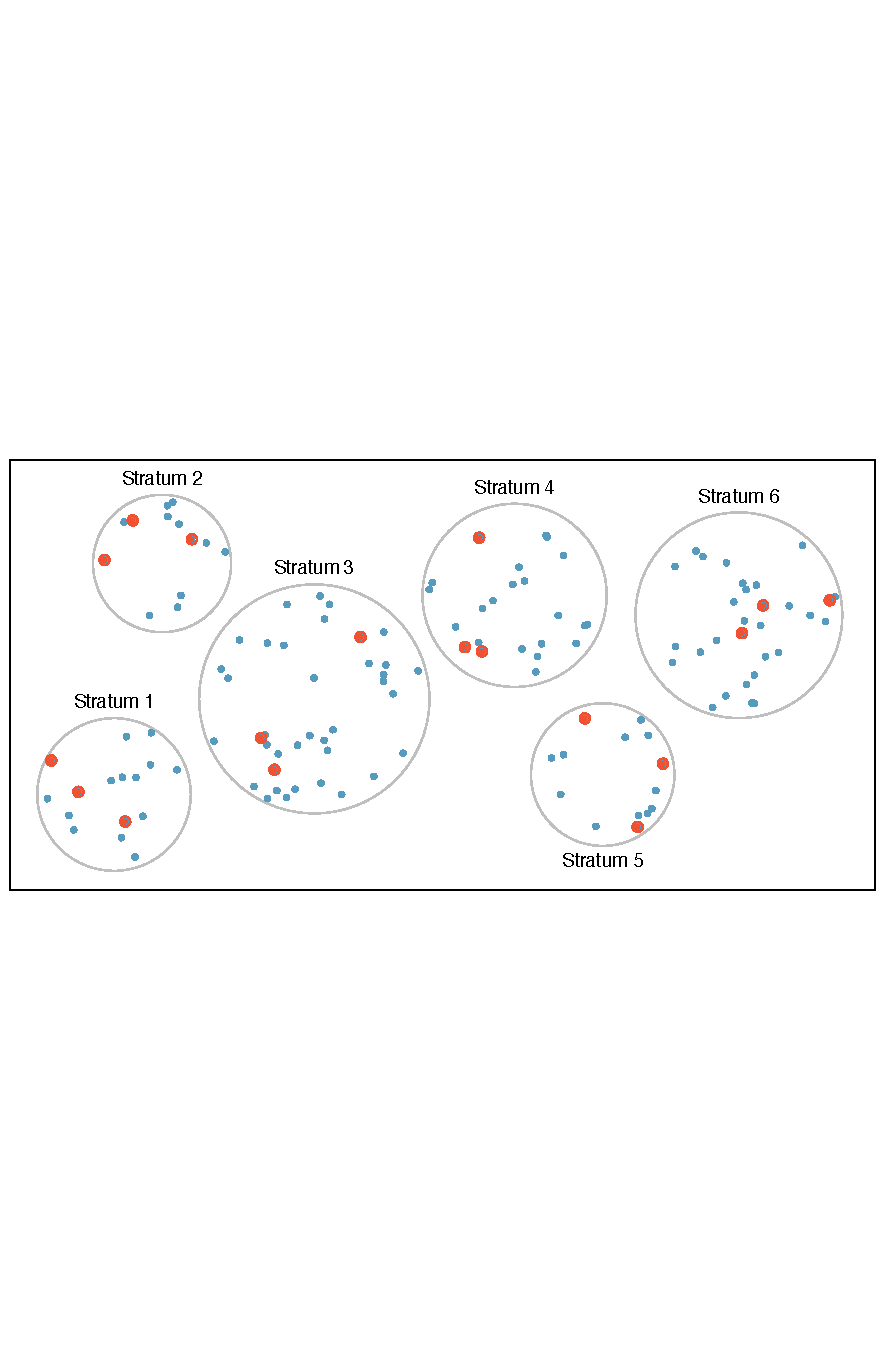
\includegraphics[width=0.9\textwidth]{1-4_obs_studies_sampling/figures/sampling_methods/stratified}
\end{center}

\end{frame}

%%%%%%%%%%%%%%%%%%%%%%%%%%%%%%%%%%%%

\begin{frame}
\frametitle{Cluster sample}

\hl{Clusters} are usually not made up of homogeneous observations, and we take a simple random sample from a random sample of clusters. Usually preferred for economical reasons.

\begin{center}
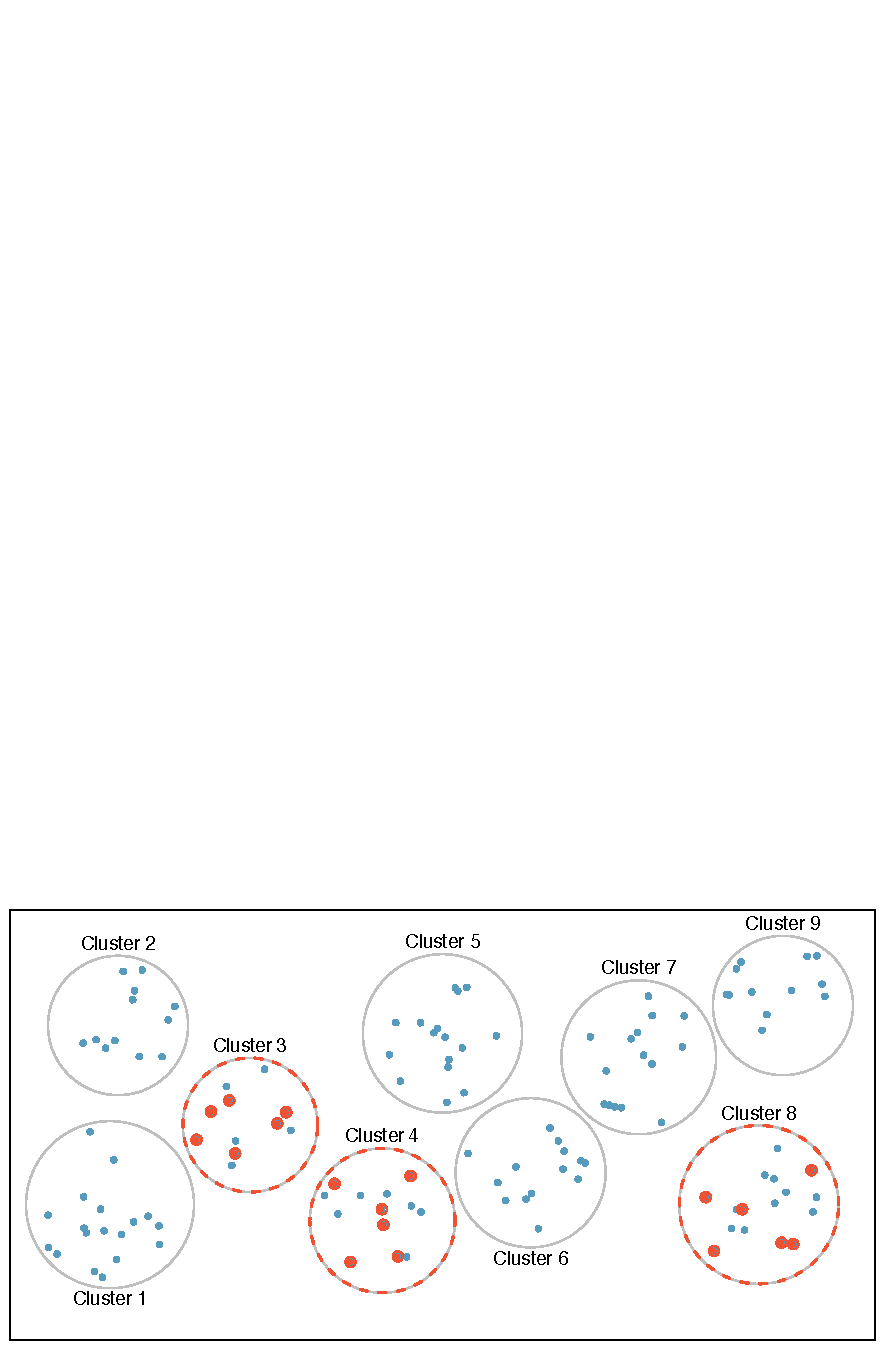
\includegraphics[width=0.9\textwidth]{1-4_obs_studies_sampling/figures/sampling_methods/cluster}
\end{center}

\end{frame}

%%%%%%%%%%%%%%%%%%%%%%%%%%%%%%%%%%%%

\begin{frame}
\frametitle{Practice}

\pq{A city council has requested a household survey be conducted in a suburban area of their city. The area is broken into many distinct and unique neighborhoods, some including large homes, some with only apartments. Which approach would likely be the \emph{least} effective?}

\begin{enumerate}[(a)]
\item Simple random sampling
\solnMult{Cluster sampling}
\item Stratified sampling
\item Blocked sampling
\end{enumerate}

\end{frame}

%%%%%%%%%%%%%%%%%%%%%%%%%%%%%%%%%%%%
%%%%%%%%%%%%%%%%%%%%%%%%%%%%%%%%%%%%

\section{Experiments}

%%%%%%%%%%%%%%%%%%%%%%%%%%%%%%%%%%%%

\begin{frame}
\frametitle{Principles of experimental design}

\begin{enumerate}

\item \hl{Control:} Compare treatment of interest to a control group.

\item \hl{Randomize:} Randomly assign subjects to treatments, and randomly sample from the population whenever possible.

\item \hl{Replicate:} Within a study, replicate by collecting a sufficiently large sample. Or replicate the entire study.

\item \hl{Block:} If there are variables that are known or suspected to affect the response variable, first group subjects into \hl{blocks} based on these variables, and then randomize cases within each block to treatment groups.

\end{enumerate}

\end{frame}

%%%%%%%%%%%%%%%%%%%%%%%%%%%%%%%%%%%%

\begin{frame}
\frametitle{More on blocking}


\twocol{0.25}{0.75}
{
\begin{center}
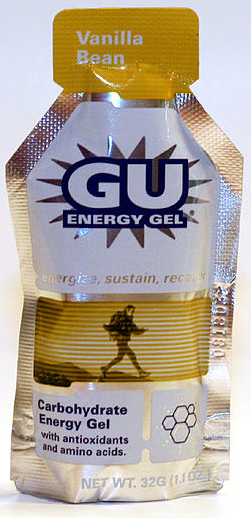
\includegraphics[width=\textwidth]{1-3_data_collection_principles/figures/gu}
\end{center}
}
{
\begin{itemize}
\item We would like to design an experiment to investigate if energy gels makes you run faster:

\pause

\begin{itemize}
\item Treatment: energy gel
\item Control: no energy gel
\end{itemize}

\pause

\item It is suspected that energy gels might affect pro and amateur athletes differently, therefore we block for pro status:

\pause

\begin{itemize}
\item Divide the sample to pro and amateur
\item Randomly assign pro athletes to treatment and control groups
\item Randomly assign amateur athletes to treatment and control groups
\item Pro/amateur status is equally represented in the resulting treatment and control groups
\end{itemize}
\end{itemize}
}

\pause

\dq{Why is this important? Can you think of other variables to block for?}

\end{frame}

%%%%%%%%%%%%%%%%%%%%%%%%%%%%%%%%%%%%

\begin{frame}
\frametitle{Practice}

\pq{A study is designed to test the effect of light level and noise level on exam performance of students. The researcher also believes that light and noise levels might have different effects on males and females, so wants to make sure both genders are equally represented in each group. Which of the below is correct?}

\begin{enumerate}[(a)]
\item There are 3 explanatory variables (light, noise, gender) and 1 response variable (exam performance)
\solnMult{There are 2 explanatory variables (light and noise), 1 blocking variable (gender), and 1 response variable (exam performance)}
\item There is 1 explanatory variable (gender) and 3 response variables (light, noise, exam performance)
\item There are 2 blocking variables (light and noise), 1 explanatory variable (gender), and 1 response variable (exam performance)
\end{enumerate}

\end{frame}

%%%%%%%%%%%%%%%%%%%%%%%%%%%%%%%%%%%%

\begin{frame}
\frametitle{Difference between blocking and explanatory variables}

\begin{itemize}

\item Factors are conditions we can impose on the experimental units.

\item Blocking variables are characteristics that the experimental units come with, that we would like to control for.

\item Blocking is like stratifying, except used in experimental settings when randomly assigning, as opposed to when sampling.

\end{itemize}

\end{frame}

%%%%%%%%%%%%%%%%%%%%%%%%%%%%%%%%%%%%

\begin{frame}
\frametitle{More experimental design terminology...}

\begin{itemize}

\item \hl{Placebo:} fake treatment, often used as the control group for medical studies

\item \hl{Placebo effect:} experimental units showing improvement simply because they believe they are receiving a special treatment

\item \hl{Blinding:} when experimental units do not know whether they are in the control or treatment group

\item \hl{Double-blind:} when both the experimental units and the researchers who interact with the patients do not know who is in the control and who is in the treatment group

\end{itemize}

\end{frame}

%%%%%%%%%%%%%%%%%%%%%%%%%%%%%%%%%%%%

\begin{frame}
\frametitle{Practice}

\pq{What is the main difference between observational studies and experiments?}

\begin{enumerate}[(a)]
\item Experiments take place in a lab while observational studies do not need to.
\item In an observational study we only look at what happened in the past.
\solnMult{Most experiments use random assignment while observational studies do not.}
\item Observational studies are completely useless since no causal inference can be made based on their findings.
\end{enumerate}

\end{frame}

%%%%%%%%%%%%%%%%%%%%%%%%%%%%%%%%%%%%

\begin{frame}
\frametitle{Random assignment vs. random sampling}

\begin{center}
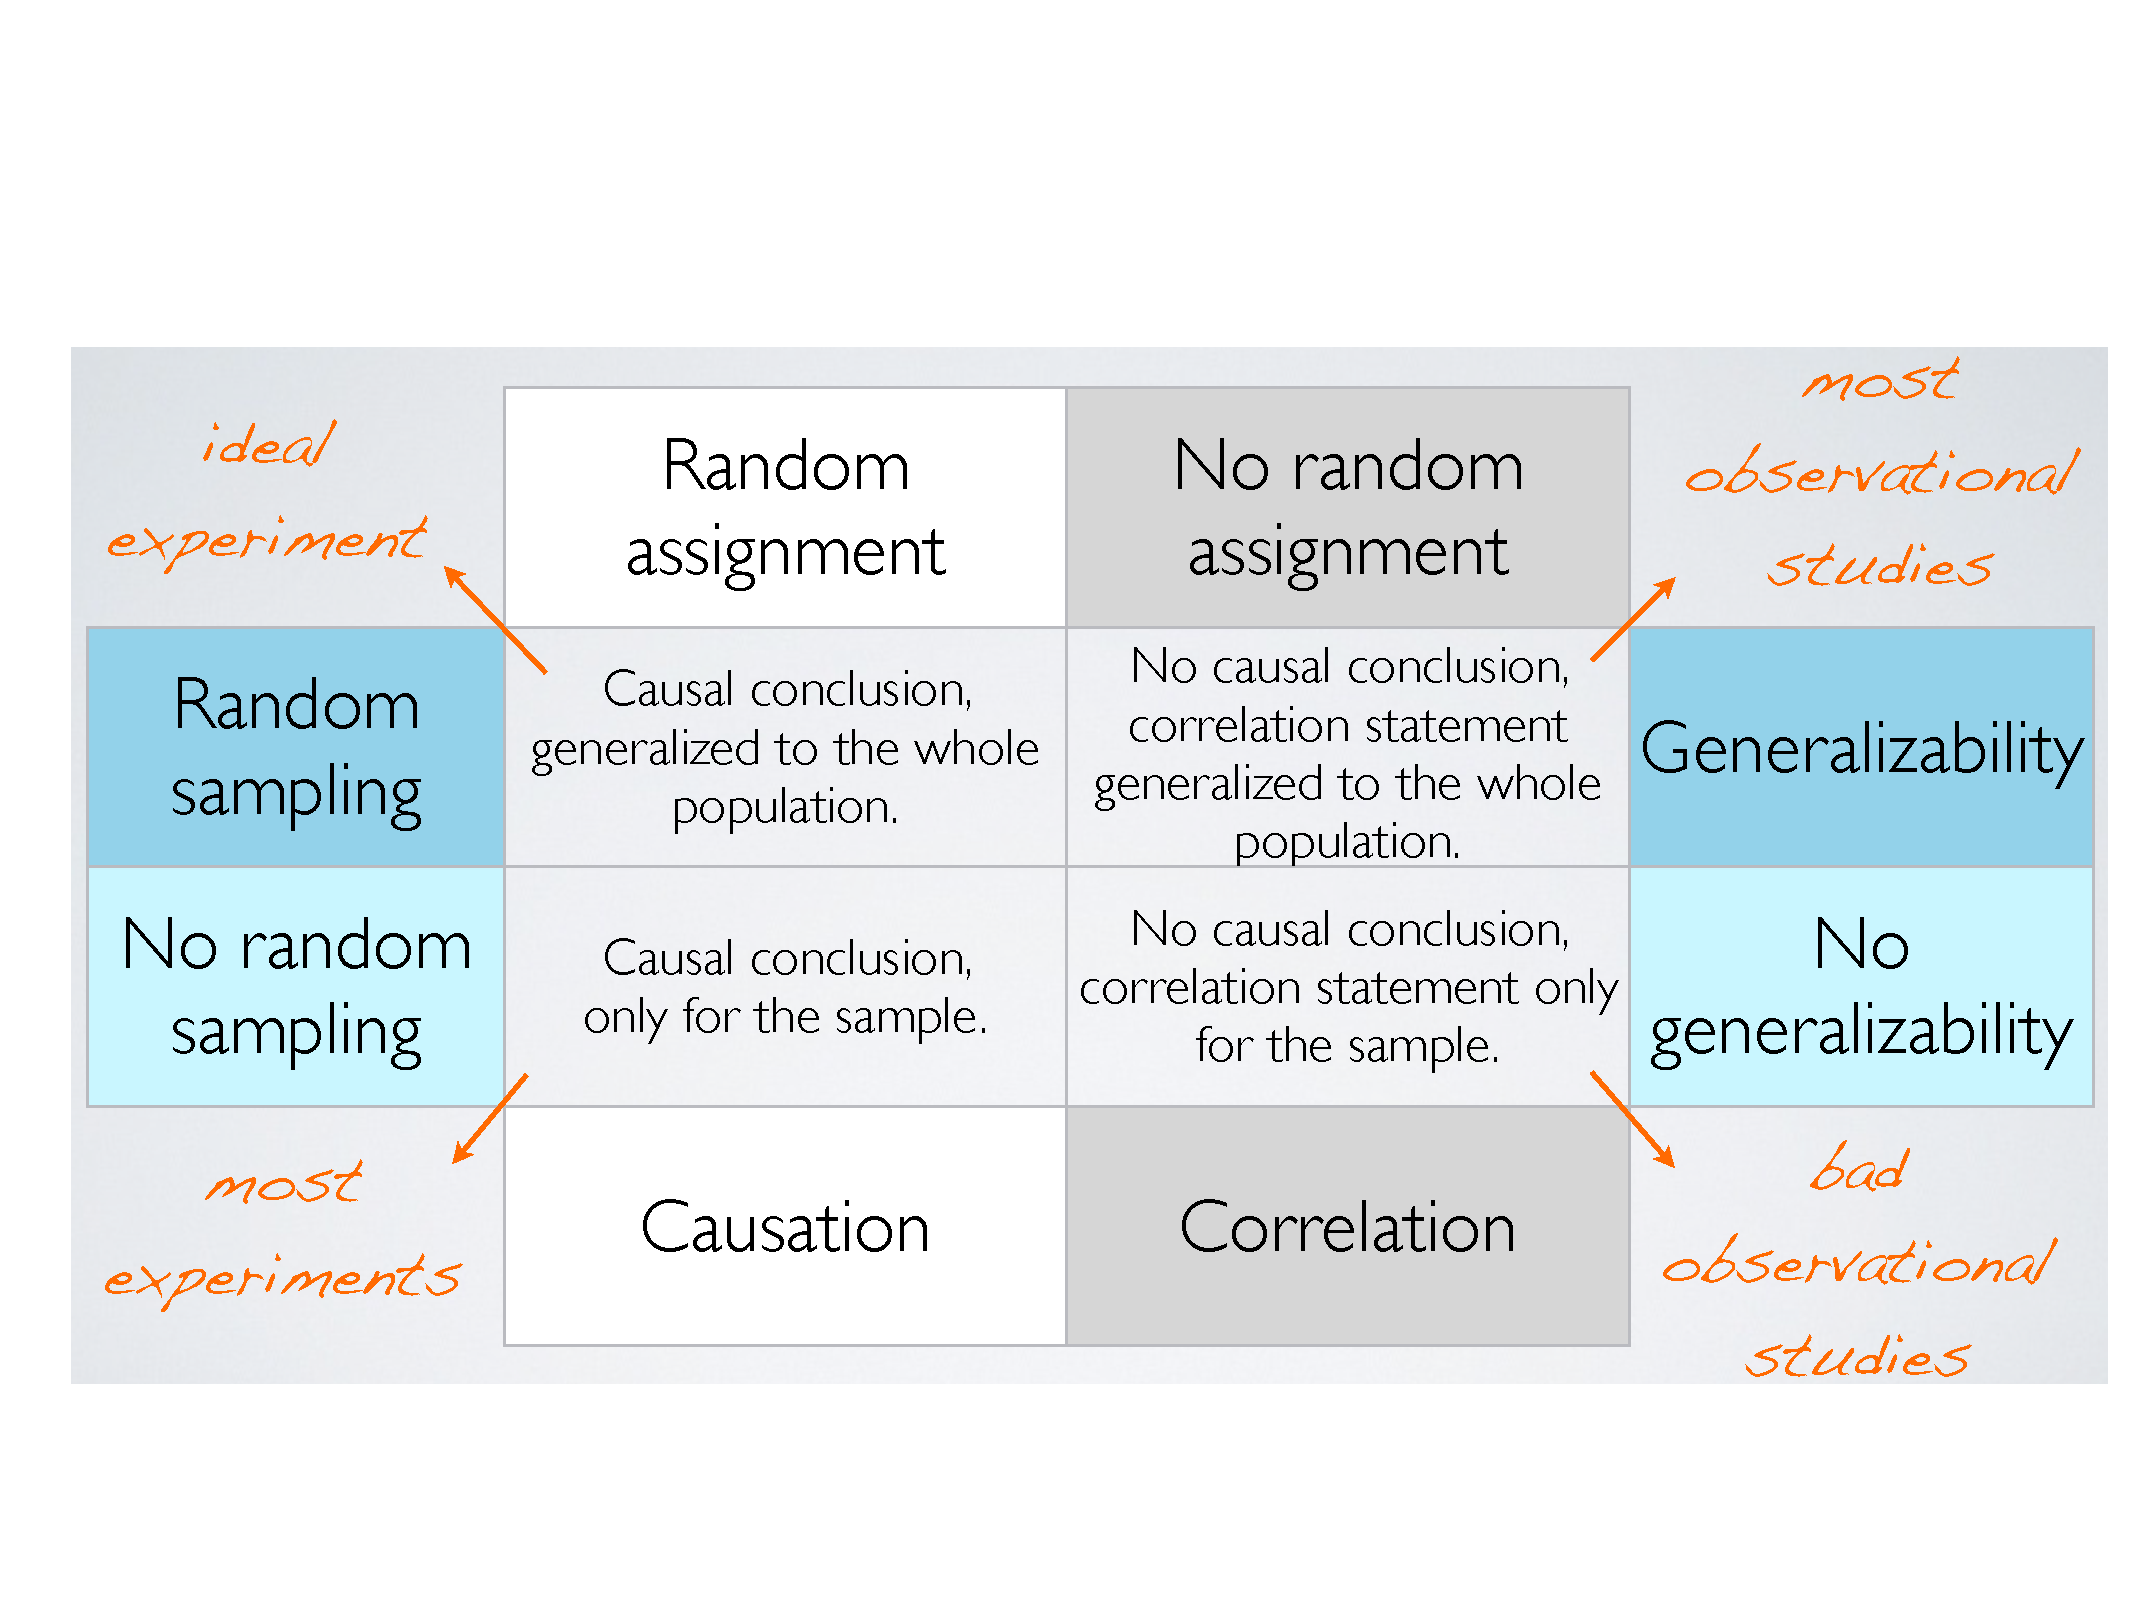
\includegraphics[width=\textwidth]{1-5_experiments/figures/random_sample_assignment}
\end{center}

\end{frame}

%%%%%%%%%%%%%%%%%%%%%%%%%%%%%%%%%%%%
%%%%%%%%%%%%%%%%%%%%%%%%%%%%%%%%%%%%

\section{Examining numerical data}

%%%%%%%%%%%%%%%%%%%%%%%%%%%%%%%%%%%%

\subsection{Scatterplots for paired data}

%%%%%%%%%%%%%%%%%%%%%%%%%%%%%%%%%%%%

\begin{frame}
\frametitle{Scatterplot}

\hl{Scatterplots} are useful for visualizing the relationship between two numerical variables.

\begin{columns}[c]

\column{0.6 \textwidth}

\dq{Do life expectancy and total fertility appear to be \hl{associated} or \hl{independent}?}

\soln{\onslide<2->{They appear to be linearly and negatively associated: as fertility increases, life expectancy decreases.}}

\dq{Was the relationship the same throughout the years, or did it change?}

\soln{\onslide<3->{The relationship changed over the years.}}

\column{0.4 \textwidth}

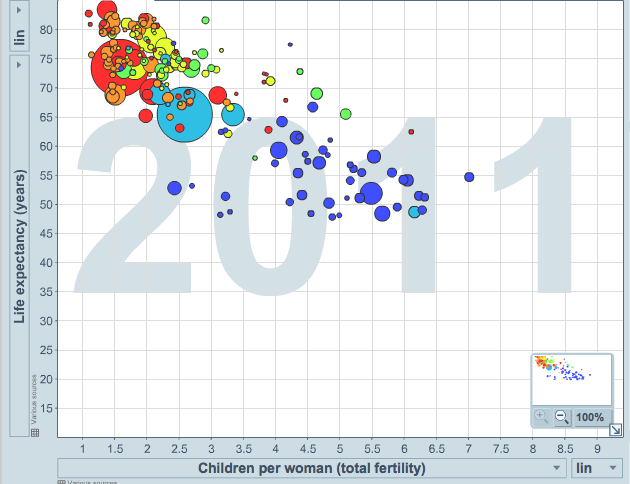
\includegraphics[width=\textwidth]{1-6_numerical_data/figures/life_exp_child}

\end{columns}

\ct{\webURL{http://www.gapminder.org/world}}

\end{frame}

%%%%%%%%%%%%%%%%%%%%%%%%%%%%%%%%%%%%

\subsection{Dot plots and the mean}

%%%%%%%%%%%%%%%%%%%%%%%%%%%%%%%%%%%%

\begin{frame}
\frametitle{Dot plots}

Useful for visualizing one numerical variable. Darker colors represent areas where there are more observations.

\begin{center}
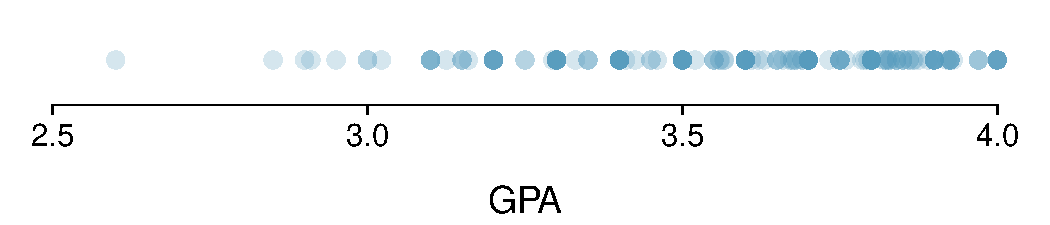
\includegraphics[width=\textwidth]{1-6_numerical_data/figures/gpa_dot_plot/gpa_dot_plot}
\end{center}

\dq{How would you describe the distribution of GPAs in this data set? Make sure to say something about the center, shape, and spread of the distribution.}

\end{frame}

%%%%%%%%%%%%%%%%%%%%%%%%%%%%%%%%%%%%


\begin{frame}
\frametitle{Dot plots \& mean}

\begin{center}
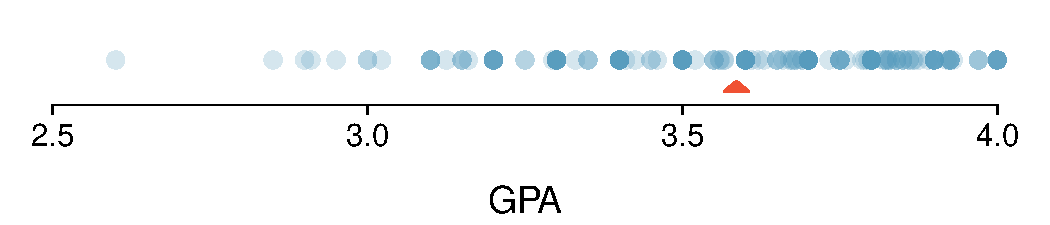
\includegraphics[width=\textwidth]{1-6_numerical_data/figures/gpa_dot_plot/gpa_dot_plot_mean}
\end{center}

\begin{itemize}

\item The \hl{mean}, also called the \hl{average} (marked with a triangle in the above plot), is one way to measure the center of a \hl{distribution} of data.

\item The mean GPA is 3.59.

\end{itemize} 

\end{frame}

%%%%%%%%%%%%%%%%%%%%%%%%%%%%%%%%%%%%

\begin{frame}
\frametitle{Mean}

\begin{itemize}

\item The \hl{sample mean}, denoted as \mathhl{\bar{x}}, can be calculated as

\[ \bar{x} = \frac{x_1 + x_2 + \cdots + x_n}{n}, \]

where $x_1, x_2, \cdots, x_n$ represent the \hl{n} observed values.

\item The \hl{population mean} is also computed the same way but is denoted as \mathhl{\mu}. It is often not possible to calculate $\mu$ since population data are rarely available.

\item The sample mean is a \hl{sample statistic}, and serves as a \hl{point estimate} of the population mean. This estimate may not be perfect, but if the sample is good (representative of the population), it is usually a pretty good estimate. 

\end{itemize}

\end{frame}

%%%%%%%%%%%%%%%%%%%%%%%%%%%%%%%%%%%%

\begin{frame}
\frametitle{Stacked dot plot}

Higher bars represent areas where there are more observations, makes it a little easier to judge the center and the shape of the distribution.

\begin{center}
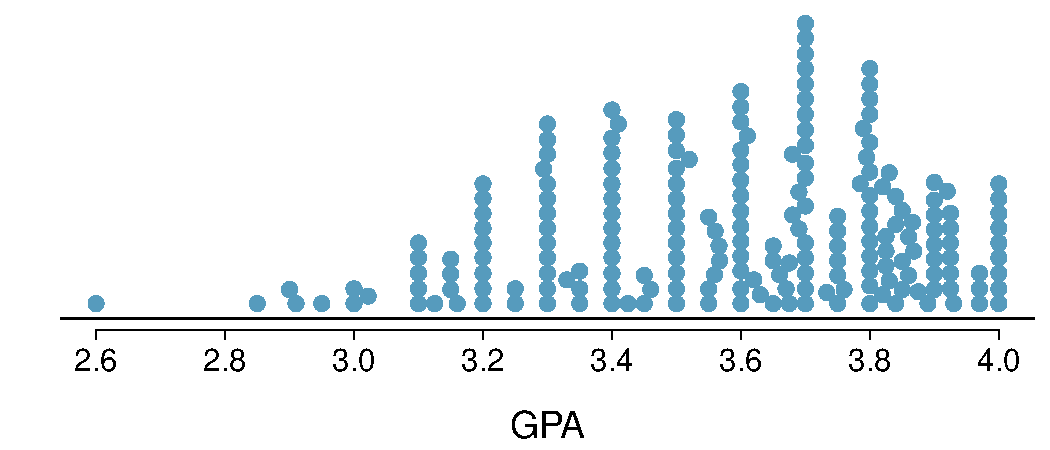
\includegraphics[width=\textwidth]{1-6_numerical_data/figures/gpa_dot_plot/gpa_dot_plot_stacked}
\end{center}

\end{frame}

%%%%%%%%%%%%%%%%%%%%%%%%%%%%%%%%%%%%

\subsection{Histograms and shape}

%%%%%%%%%%%%%%%%%%%%%%%%%%%%%%%%%%%%

\begin{frame}[fragile]
\frametitle{Histograms - Extracurricular hours}

\begin{itemize}

\item Histograms provide a view of the \hl{data density}. Higher bars represent where the data are relatively more common.

\item Histograms are especially convenient for describing the \hl{shape} of the data distribution.

\item The chosen \hl{bin width} can alter the story the histogram is telling.

\end{itemize}

\begin{center}
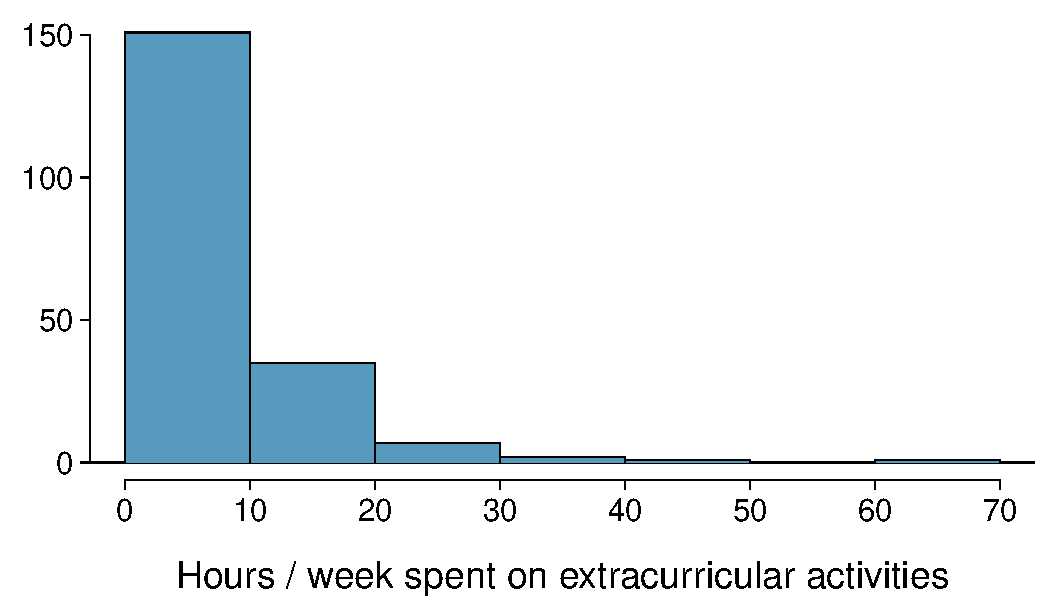
\includegraphics[width=0.75\textwidth]{1-6_numerical_data/figures/extracurr_hrs_hist/extracurr_hrs_hist}
\end{center}

\end{frame}

%%%%%%%%%%%%%%%%%%%%%%%%%%%%%%%%%%%%

\begin{frame}
\frametitle{Bin width}

\dq{Which one(s) of these histograms are useful? Which reveal too much about the data? Which hide too much?}

\begin{center}
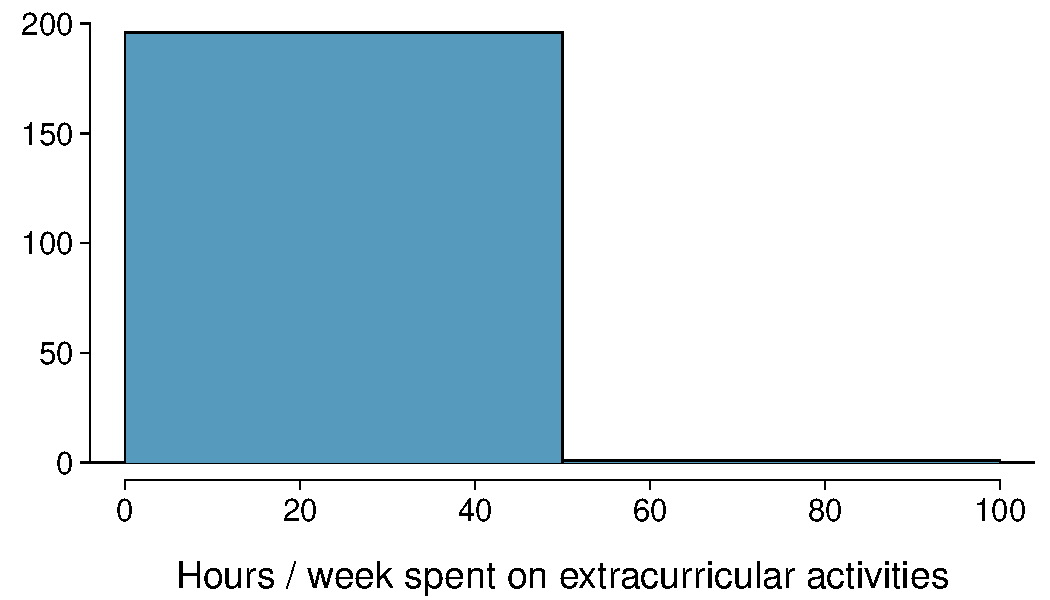
\includegraphics[width=0.45\textwidth]{1-6_numerical_data/figures/extracurr_hrs_hist/extracurr_hrs_hist2}
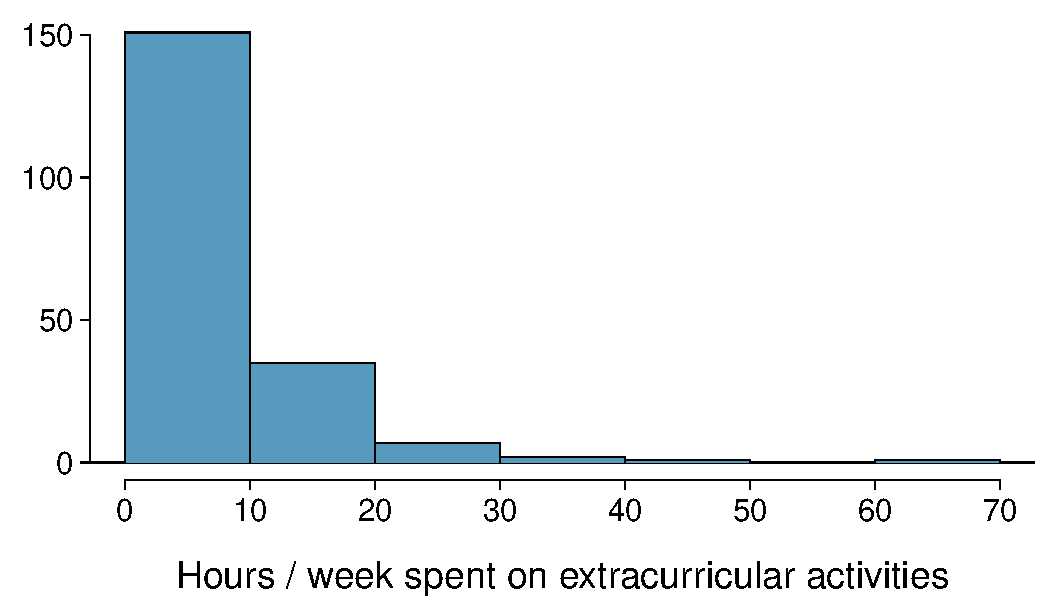
\includegraphics[width=0.45\textwidth]{1-6_numerical_data/figures/extracurr_hrs_hist/extracurr_hrs_hist} \\
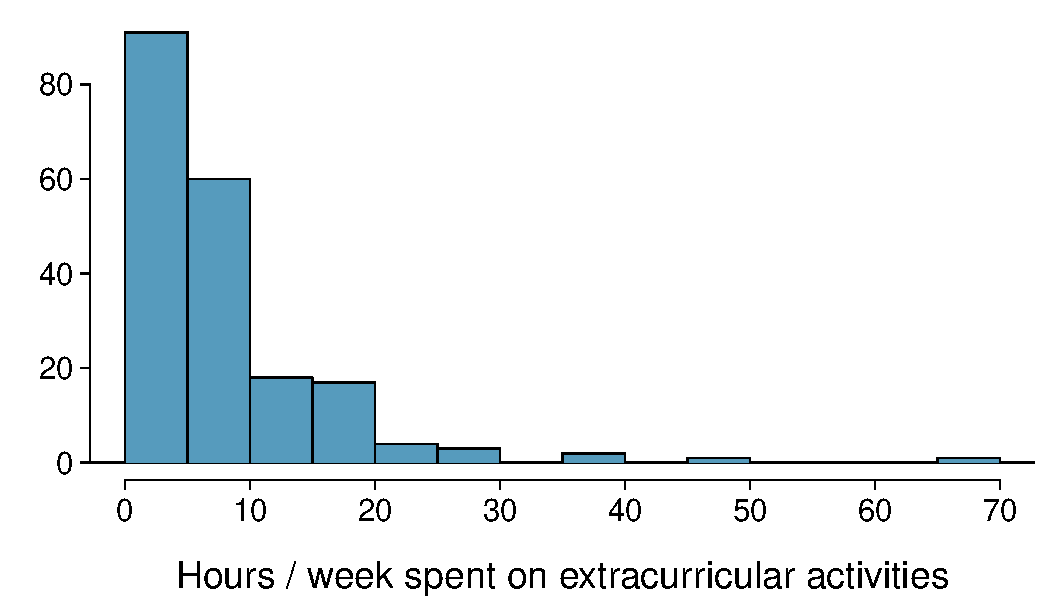
\includegraphics[width=0.45\textwidth]{1-6_numerical_data/figures/extracurr_hrs_hist/extracurr_hrs_hist20}
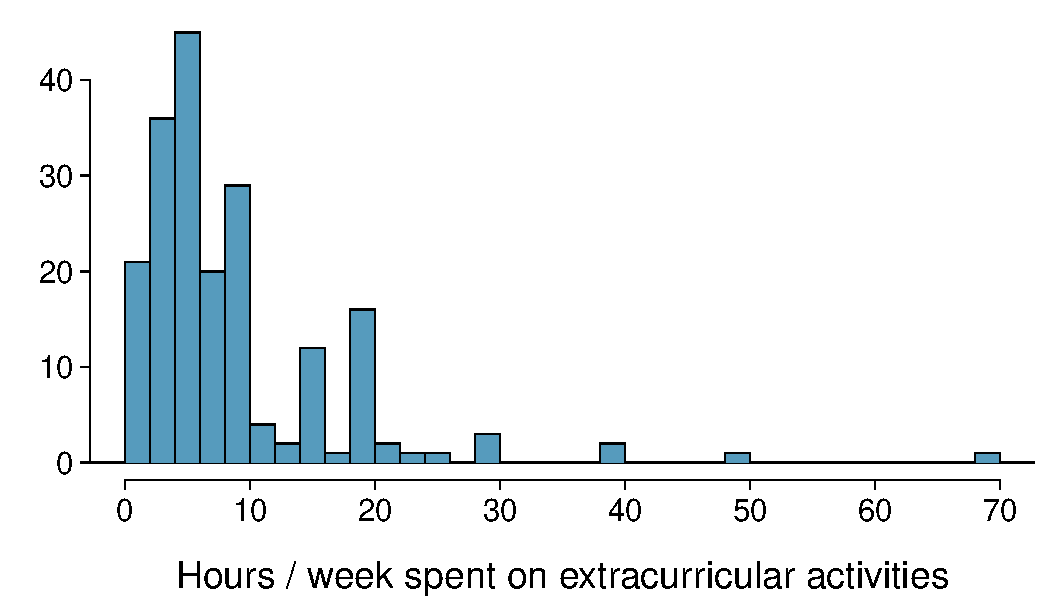
\includegraphics[width=0.45\textwidth]{1-6_numerical_data/figures/extracurr_hrs_hist/extracurr_hrs_hist30}
\end{center}

\end{frame}

%%%%%%%%%%%%%%%%%%%%%%%%%%%%%%%%%%%%

\begin{frame}
\frametitle{Shape of a distribution: modality}

Does the histogram have a single prominent peak (\hl{unimodal}), several prominent peaks (\hl{bimodal/multimodal}), or no apparent peaks (\hl{uniform})?

\begin{center}
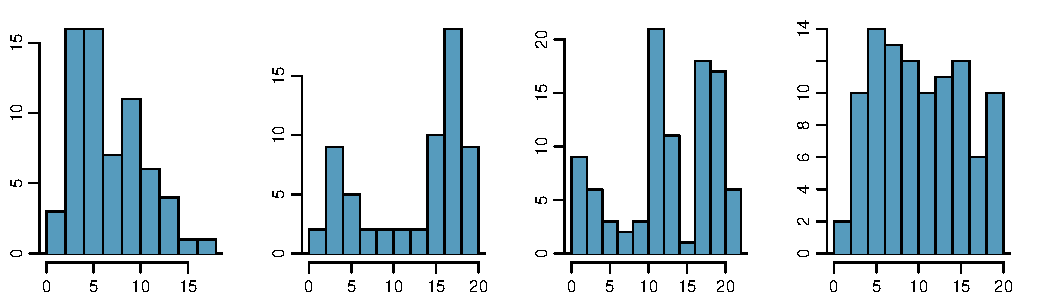
\includegraphics[width=0.75\textwidth]{1-6_numerical_data/figures/singleBiMultiModalUnifPlots/singleBiMultiModalUnifPlots}
\end{center}

\Note{In order to determine modality, step back and imagine a smooth curve over the histogram -- imagine that the bars are wooden blocks and you drop a limp spaghetti over them, the shape the spaghetti would take could be viewed as a smooth curve.}

\end{frame}

%%%%%%%%%%%%%%%%%%%%%%%%%%%%%%%%%%%%

\begin{frame}
\frametitle{Shape of a distribution: skewness}

Is the histogram \hl{right skewed}, \hl{left skewed}, or \hl{symmetric}?

\begin{center}
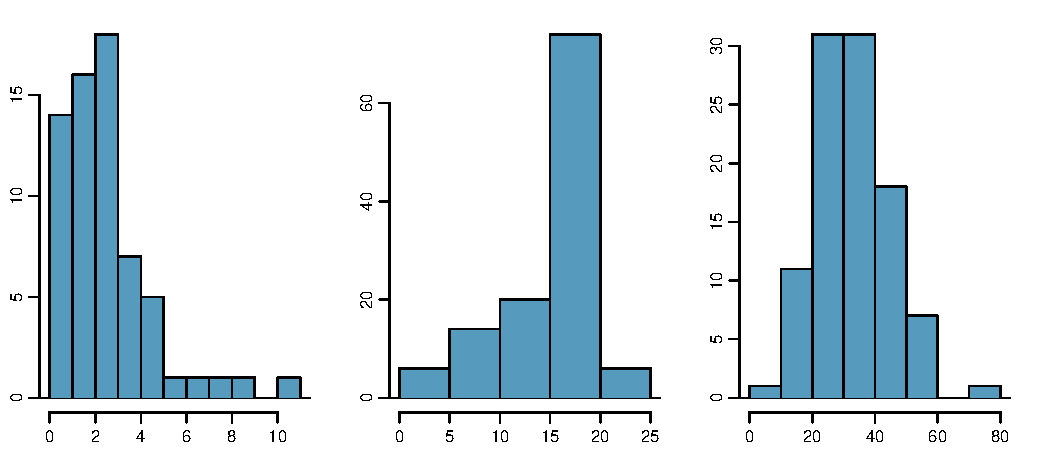
\includegraphics[width=0.8\textwidth]{1-6_numerical_data/figures/skewedSymPlots/skewedSymPlots}
\end{center}

\Note{Histograms are said to be skewed to the side of the long tail.}

\end{frame}

%%%%%%%%%%%%%%%%%%%%%%%%%%%%%%%%%%%%

\begin{frame}
\frametitle{Shape of a distribution: unusual observations}

Are there any unusual observations or potential \hl{outliers}?

\begin{center}
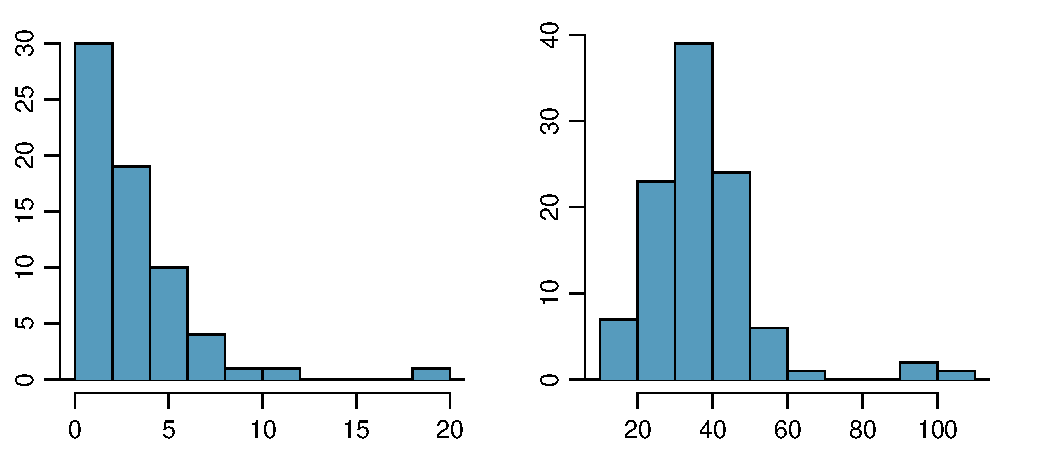
\includegraphics[width=0.8\textwidth]{1-6_numerical_data/figures/outlierPlots/outlierPlots}
\end{center}

\end{frame}

%%%%%%%%%%%%%%%%%%%%%%%%%%%%%%%%%%%%

\begin{frame}
\frametitle{Extracurricular activities}

\dq{How would you describe the shape of the distribution of hours per week students spend on extracurricular activities?}

\begin{center}
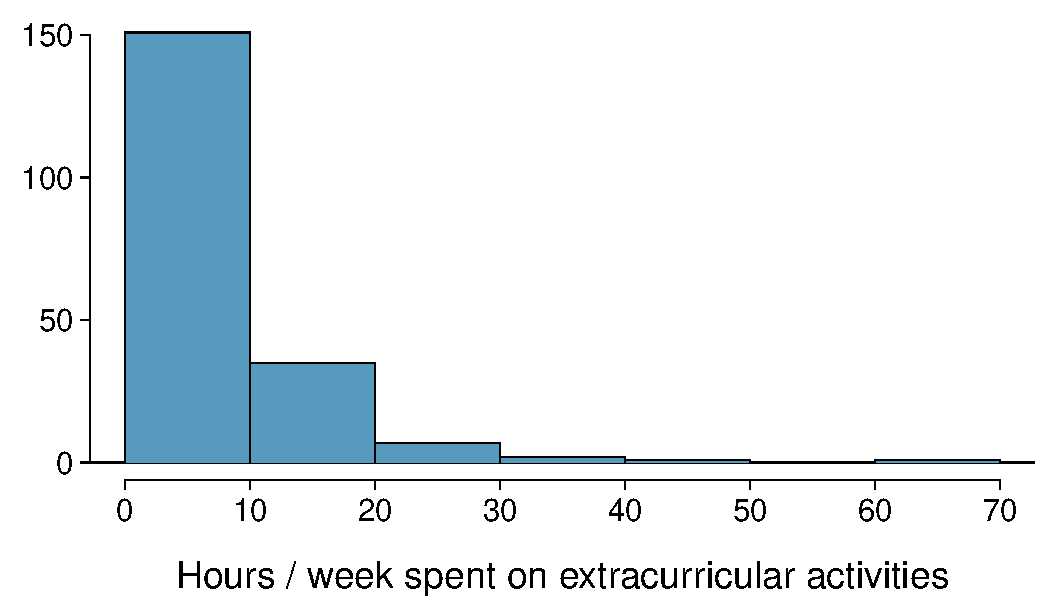
\includegraphics[width=0.75\textwidth]{1-6_numerical_data/figures/extracurr_hrs_hist/extracurr_hrs_hist}
\end{center}

\soln{\pause{Unimodal and right skewed, with a potentially unusual observation at 60 hours/week.}}

\end{frame}

%%%%%%%%%%%%%%%%%%%%%%%%%%%%%%%%%%%%

\begin{frame}
\frametitle{Commonly observed shapes of distributions}

\begin{itemize}

\item modality \\
$\:$ \\
\pause

\begin{columns}[c]
\column{0.25\textwidth}
unimodal \\
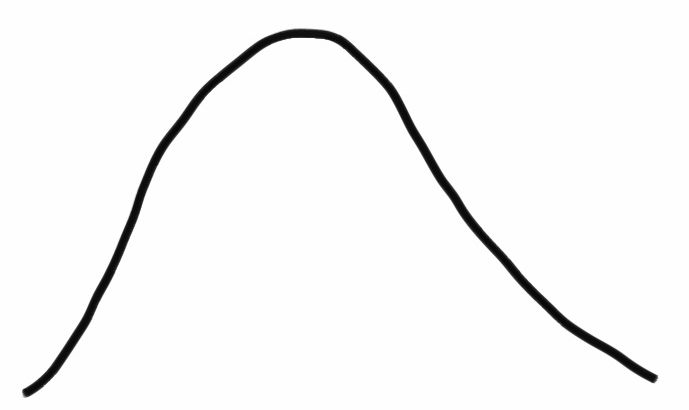
\includegraphics[width=\textwidth]{1-6_numerical_data/figures/shape_sketches/unimodal} 
\pause
\column{0.25\textwidth}
bimodal \\
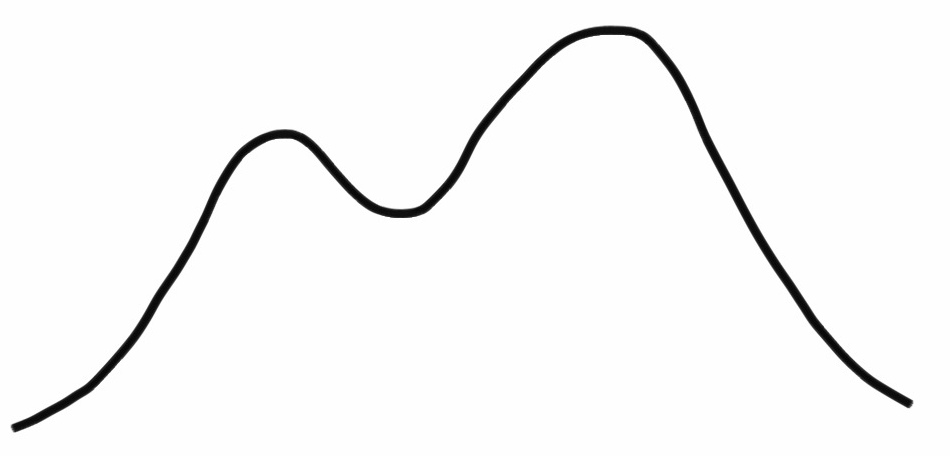
\includegraphics[width=\textwidth]{1-6_numerical_data/figures/shape_sketches/bimodal} 
\pause
\column{0.25\textwidth}
multimodal \\

\includegraphics[width=\textwidth]{1-6_numerical_data/figures/shape_sketches/multimodal} 
\pause
\column{0.25\textwidth}
uniform
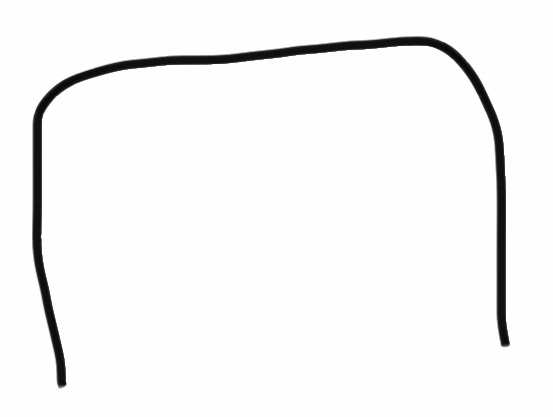
\includegraphics[width=\textwidth]{1-6_numerical_data/figures/shape_sketches/uniform} 
\end{columns}

\pause

$\:$ \\

\item skewness \\
$\:$ \\
\pause

\begin{columns}[c]
\column{0.25\textwidth}
right skew \\
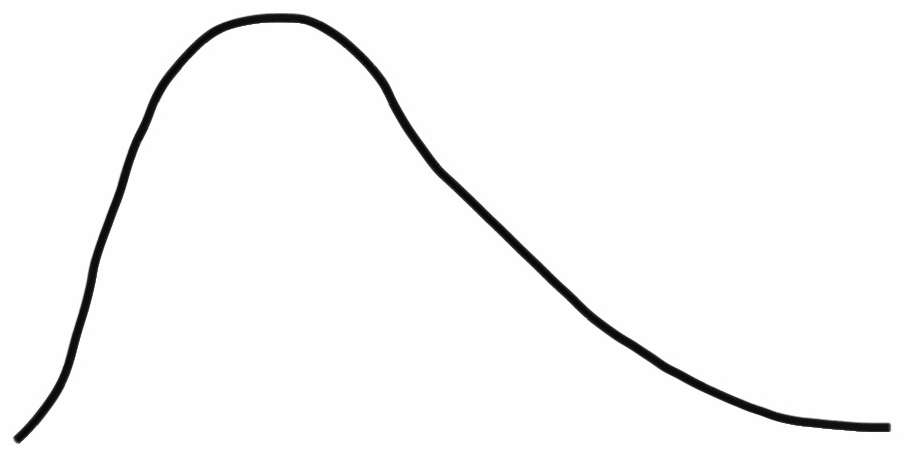
\includegraphics[width=\textwidth]{1-6_numerical_data/figures/shape_sketches/right_skew} 
\pause
\column{0.25\textwidth}
left skew \\
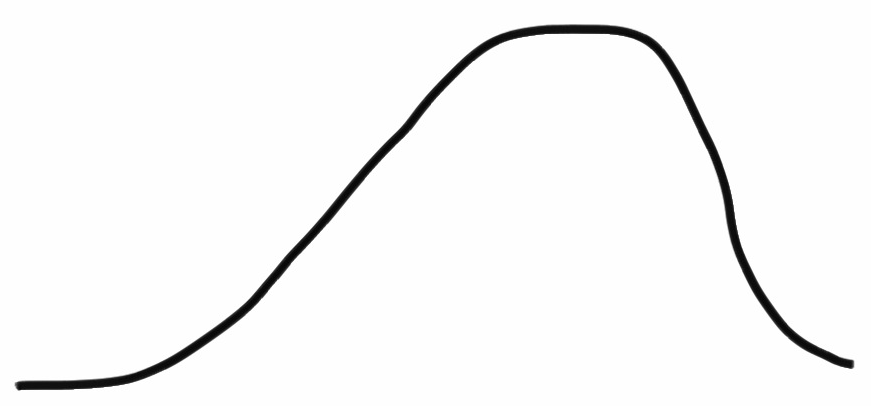
\includegraphics[width=\textwidth]{1-6_numerical_data/figures/shape_sketches/left_skew} 
\pause
\column{0.25\textwidth}
symmetric \\
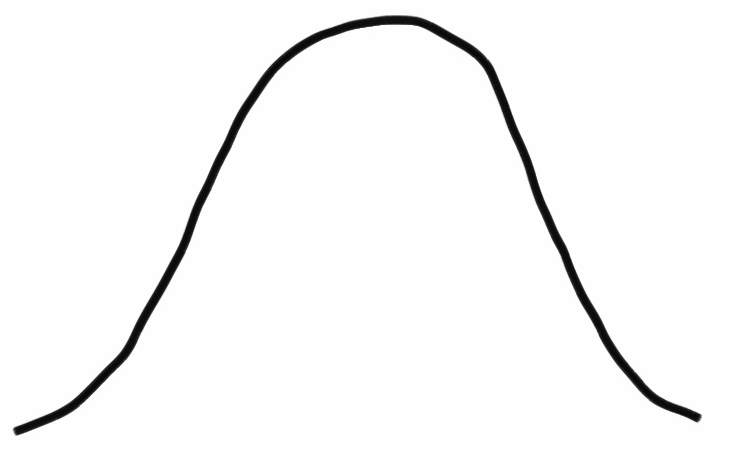
\includegraphics[width=\textwidth]{1-6_numerical_data/figures/shape_sketches/symmetric} 
\end{columns}

\end{itemize}

\end{frame}

%%%%%%%%%%%%%%%%%%%%%%%%%%%%%%%%%%%

\begin{frame}
\frametitle{Practice}

\pq{Which of these variables do you expect to be uniformly distributed?}

\begin{enumerate}[(a)]
\item weights of adult females
\item salaries of a random sample of people from North Carolina
\item house prices
\solnMult{birthdays of classmates (day of the month)}
\end{enumerate}

\end{frame}

%%%%%%%%%%%%%%%%%%%%%%%%%%%%%%%%%%%

\begin{frame}
\frametitle{Application activity: Shapes of distributions}

\app{Sketch the expected distributions of the following variables:
\begin{itemize}
\item number of piercings
\item scores on an exam
\item IQ scores
\end{itemize}
Come up with a concise way (1-2 sentences) to teach someone how to determine the expected distribution of any variable.
}

\end{frame}

%%%%%%%%%%%%%%%%%%%%%%%%%%%%%%%%%%%

\begin{frame}
\frametitle{Are you typical?}

\begin{center}
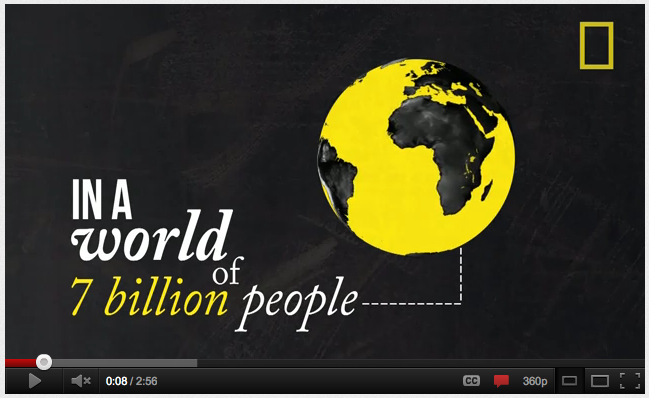
\includegraphics[width=0.75\textwidth]{1-6_numerical_data/figures/typical}
\end{center}

\begin{center}
\footnotesize{\webURL{http://www.youtube.com/watch?v=4B2xOvKFFz4}}
\end{center}

\pause

\dq{How useful are centers alone for conveying the true characteristics of a distribution?}

\end{frame}

%%%%%%%%%%%%%%%%%%%%%%%%%%%%%%%%%%%%

\subsection{Variance and standard deviation}

%%%%%%%%%%%%%%%%%%%%%%%%%%%%%%%%%%%

\begin{frame}
\frametitle{Variance}

\hl{Variance} is roughly the average squared deviation from the mean.

\formula{
\[ s^2 = \frac{\sum_{i = 1}^n (x_i - \bar{x})^2}{n - 1} \]
}

\pause

\twocol{0.5}{0.5}
{
\begin{itemize}

\item The sample mean is $\bar{x} = 6.71$, and the sample size is $n = 217$.

\onslide<3->{\item The variance of amount of sleep students get per night can be calculated as:}
\end{itemize}
}
{
\onslide<2->{
\begin{center}
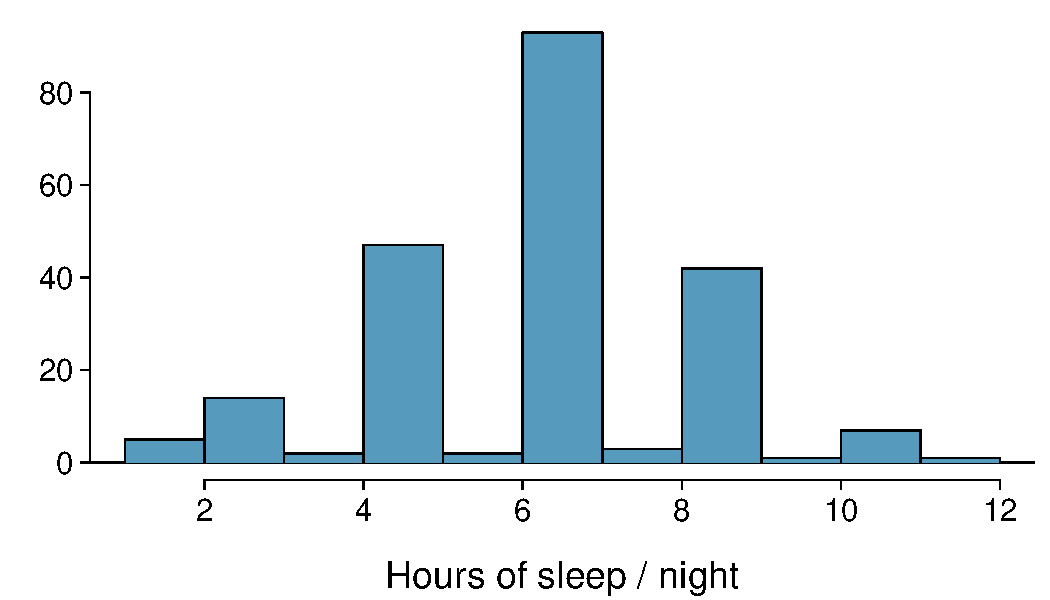
\includegraphics[width=\textwidth]{1-6_numerical_data/figures/sleep_hist/sleep_hist}
\end{center}
}
}
$\:$
\onslide<3->{
\[ s^2 = \frac{(5 - 6.71)^2 + (9 - 6.71)^2 + \cdots + (7 - 6.71)^2}{217 - 1} = 4.11~hours^2 \]
}



\end{frame}

%%%%%%%%%%%%%%%%%%%%%%%%%%%%%%%%%%%

\begin{frame}
\frametitle{Variance (cont.)}

\dq{Why do we use the squared deviation in the calculation of variance?}

\soln{\pause
\begin{itemize}
\item To get rid of negatives so that observations equally distant from the mean are weighed equally.
\item To weigh larger deviations more heavily.
\end{itemize}
}

\end{frame}

%%%%%%%%%%%%%%%%%%%%%%%%%%%%%%%%%%

\begin{frame}
\frametitle{Standard deviation}

The \hl{standard deviation} is the square root of the variance, and has the same units as the data.s

\formula{
\[ s = \sqrt{s^2} \]
}

\pause

\twocol{0.5}{0.5}
{
\begin{itemize}

\item The standard deviation of amount of sleep students get per night can be calculated as:
\[ s = \sqrt{4.11} = 2.03~hours\]

\onslide<3->{\item We can see that all of the data are within 3 standard deviations of the mean.}
\end{itemize}
}
{
\onslide<2->{
\begin{center}
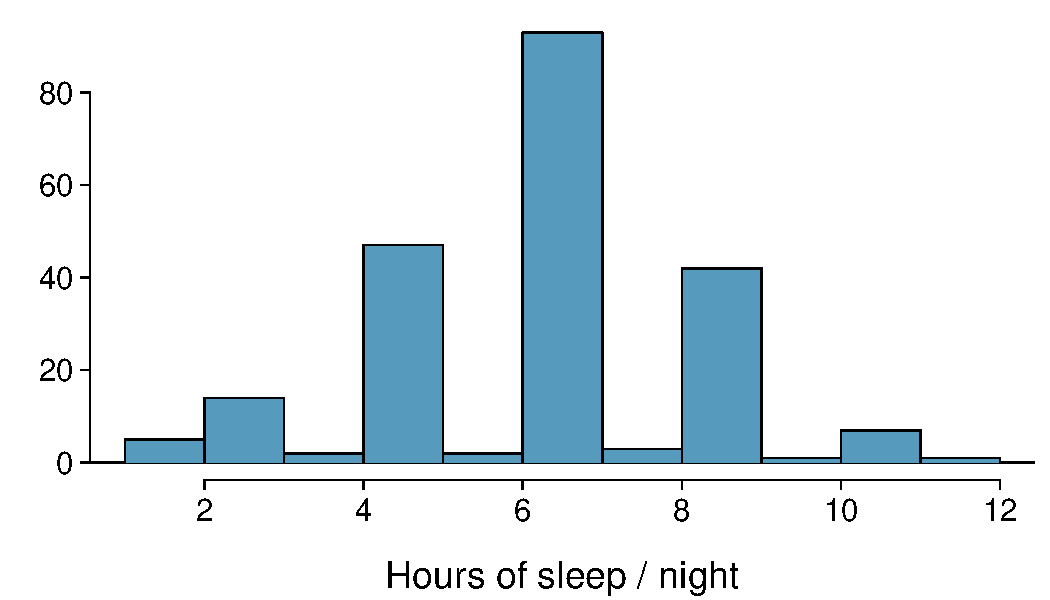
\includegraphics[width=\textwidth]{1-6_numerical_data/figures/sleep_hist/sleep_hist}
\end{center}
}
}

\end{frame}

%%%%%%%%%%%%%%%%%%%%%%%%%%%%%%%%%%%%

\subsection{Box plots, quartiles, and the median}

%%%%%%%%%%%%%%%%%%%%%%%%%%%%%%%%%%%%

\begin{frame}
\frametitle{Median}

\begin{itemize}

\item The \hl{median} is the value that splits the data in half when ordered in ascending order.

\[ 0,1,\red{2},3,4 \]

\item If there are an even number of observations, then the median is the average of the two values in the middle.

\[ 0,1,\underline{2,3},4,5 \rightarrow \frac{2 + 3}{2} = \red{2.5} \]

\item Since the median is the midpoint of the data, 50\% of the values are below it. Hence, it is also the \hl{$50^{th}$ percentile}.

\end{itemize}

\end{frame}

%%%%%%%%%%%%%%%%%%%%%%%%%%%%%%%%%%%%

\begin{frame}[fragile]
\frametitle{Q1, Q3, and IQR}

\begin{itemize}

\item The $25^{th}$ percentile is also called the first quartile, \hl{Q1}.

\item The $50^{th}$ percentile is also called the median.

\item The $75^{th}$ percentile is also called the third quartile, \hl{Q3}.

\item Between Q1 and Q3 is the middle 50\% of the data. The range these data span is called the \hl{interquartile range}, or the \hl{IQR}.
\formula{\[ IQR = Q3 - Q1 \]}
\end{itemize}

\end{frame}

%%%%%%%%%%%%%%%%%%%%%%%%%%%%%%%%%%%%

\begin{frame}
\frametitle{Box plot}

The box in a \hl{box plot} represents the middle 50\% of the data, and the thick line in the box is the median.

\begin{center}
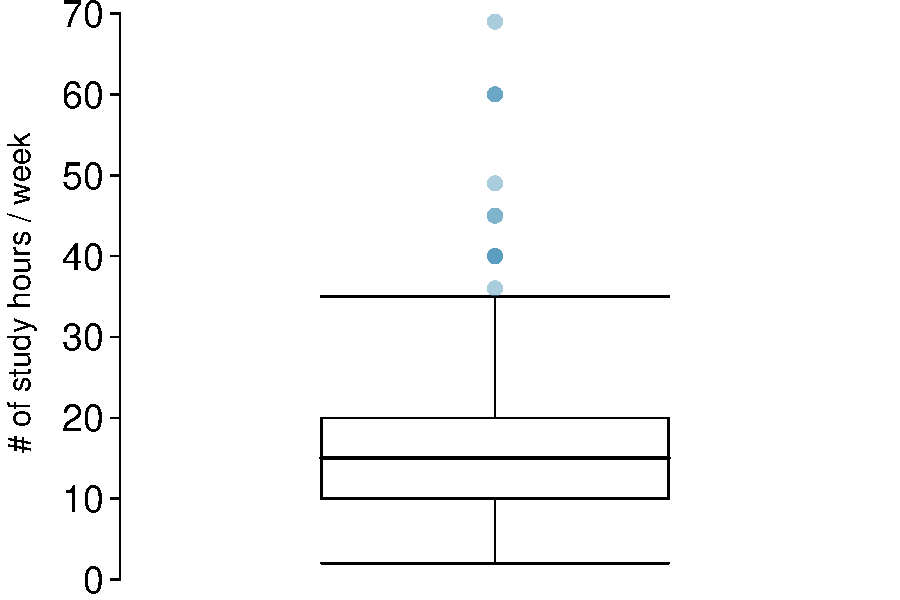
\includegraphics[width=0.7\textwidth]{1-6_numerical_data/figures/study_hours/study_hours_box}
\end{center}

\end{frame}

%%%%%%%%%%%%%%%%%%%%%%%%%%%%%%%%%%%%

\begin{frame}
\frametitle{Anatomy of a box plot}

\begin{center}
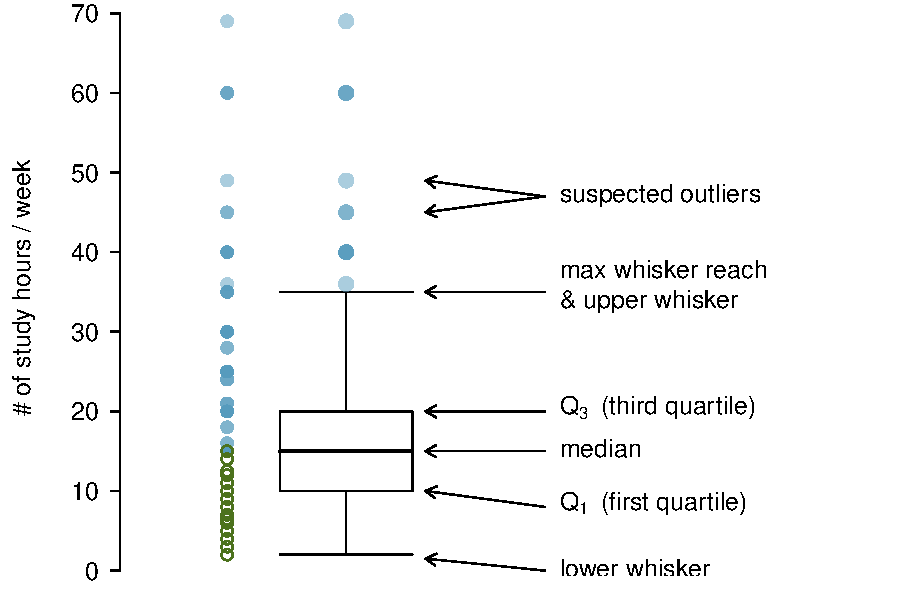
\includegraphics[width=0.95\textwidth]{1-6_numerical_data/figures/study_hours/study_hours_box_layout}
\end{center}

\end{frame}

%%%%%%%%%%%%%%%%%%%%%%%%%%%%%%%%%%%%

\begin{frame}[fragile]
\frametitle{Whiskers and outliers}

\begin{itemize}

\item \hl{Whiskers} of a box plot can extend up to $1.5 \times IQR$ away from the quartiles.
\formula{
\vspace{-0.5cm}
\begin{align*} 
\text{max~upper~whisker~reach} &= Q3 + 1.5 \times IQR \\
\text{max~lower~whisker~reach} &= Q1 - 1.5 \times IQR
\end{align*}
}
\pause
\vspace{-0.5cm}
{\small
\begin{align*}
\text{IQR}&: 20 - 10 = 10 \\
\text{max~upper~whisker~reach}&= 20 + 1.5 \times 10 = 35 \\
\text{max~lower~whisker~reach}&= 10 - 1.5 \times 10 = -5
\end{align*}
}

\pause
\vspace{-0.25cm}
\item A potential \hl{outlier} is defined as an observation beyond the maximum reach of the whiskers. It is an observation that appears extreme relative to the rest of the data.

\end{itemize}

\end{frame}

%%%%%%%%%%%%%%%%%%%%%%%%%%%%%%%%%%%%

\begin{frame}
\frametitle{Outliers (cont.)}

\dq{Why is it important to look for outliers?}

\soln{
\onslide<2->{
\begin{itemize}
\item Identify extreme skew in the distribution.
\item Identify data collection and entry errors.
\item Provide insight into interesting features of the data.
\end{itemize}
}
}

\end{frame}

%%%%%%%%%%%%%%%%%%%%%%%%%%%%%%%%%%%%

\subsection{Robust statistics}

%%%%%%%%%%%%%%%%%%%%%%%%%%%%%%%%%%%%

\begin{frame}
\frametitle{Extreme observations}

\dq{How would sample statistics such as mean, median, SD, and IQR of household income be affected if the largest value was replaced with \$10 million? What if the smallest value was replaced with \$10 million?}

\begin{center}
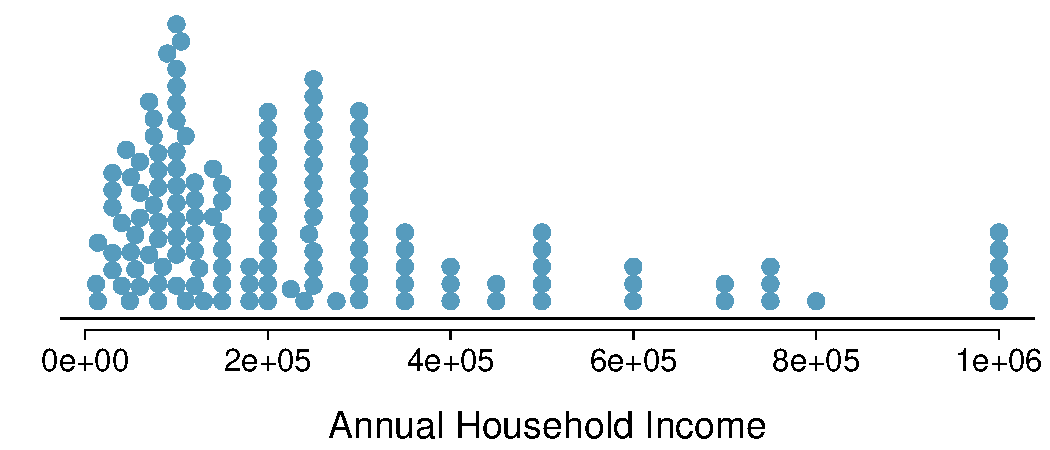
\includegraphics[width=\textwidth]{1-6_numerical_data/figures/house_income/house_income_dot_stacked}
\end{center}

\end{frame}

%%%%%%%%%%%%%%%%%%%%%%%%%%%%%%%%%%%%

\begin{frame}
\frametitle{Robust statistics}

\begin{center}
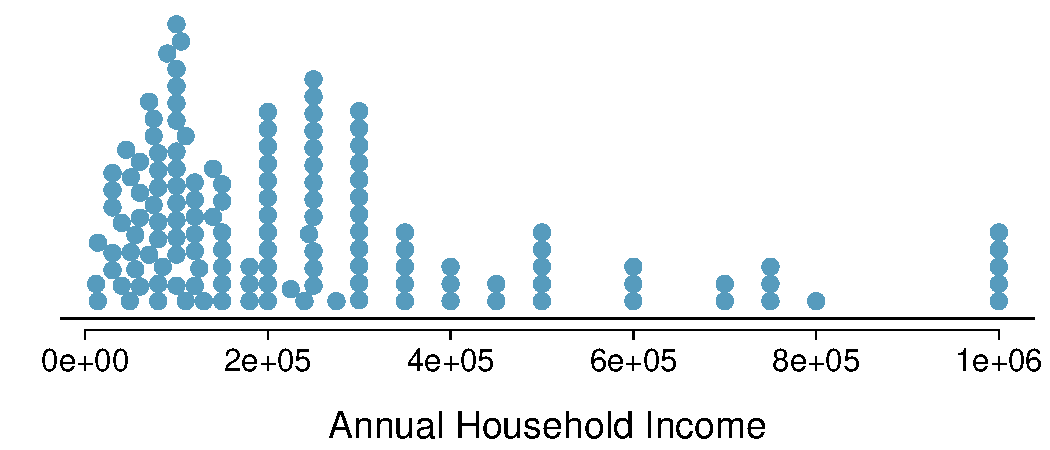
\includegraphics[width=\textwidth]{1-6_numerical_data/figures/house_income/house_income_dot_stacked}
\end{center}

{\small
\begin{center}
\begin{tabular}{l c cc c cc}
  \hline
& \hspace{0mm} & \multicolumn{2}{c}{\bf robust} & \hspace{2mm} & \multicolumn{2}{c}{\bf not robust} \\
scenario && median & IQR && $\bar{x}$ & $s$ \\ 
  \hline
original data && 190K & 200K && 245K & 226K \\ 
move largest to \$10 million && 190K & 200K && 309K & 853K \\ 
move smallest to \$10 million && 200K & 200K && 316K & 854K \\ 
   \hline
\end{tabular}
\end{center}
}

\end{frame}

%%%%%%%%%%%%%%%%%%%%%%%%%%%%%%%%%%%%

\begin{frame}
\frametitle{Robust statistics}

Median and IQR are more robust to skewness and outliers than mean and SD. Therefore,

\begin{itemize}
\item for skewed distributions it is often more helpful to use median and IQR to describe the center and spread
\item for symmetric distributions it is often more helpful to use the mean and SD to describe the center and spread
\end{itemize}

$\:$ \\

\pause

\dq{If you would like to estimate the typical household income for a student, would you be more interested in the mean or median income?}

\soln{\pause{Median}}

\end{frame}

%%%%%%%%%%%%%%%%%%%%%%%%%%%%%%%%%%%%

\begin{frame}
\frametitle{Mean vs. median}

\begin{itemize}

\item If the distribution is symmetric, center is often defined as the mean: mean $\approx$ median

\begin{center}
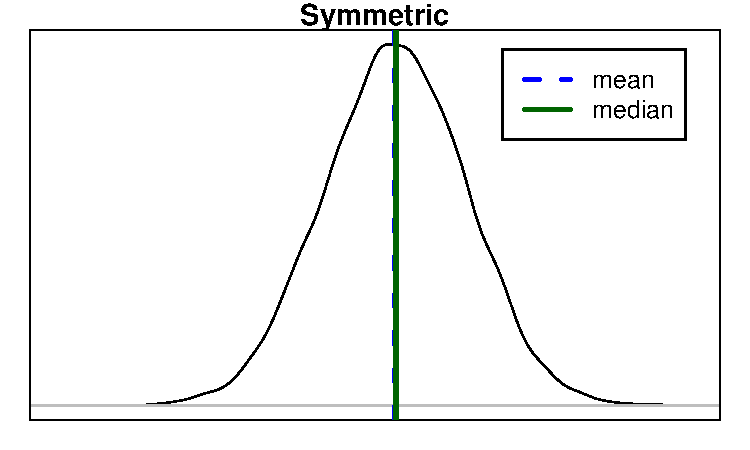
\includegraphics[width=0.33\textwidth]{1-6_numerical_data/figures/mean_med/sym}
\end{center}

\item If the distribution is skewed or has extreme outliers, center is often defined as the median
\begin{itemize}
\item Right-skewed: mean $>$ median
\item Left-skewed: mean $<$ median \\
\end{itemize}

\end{itemize}

\begin{center}
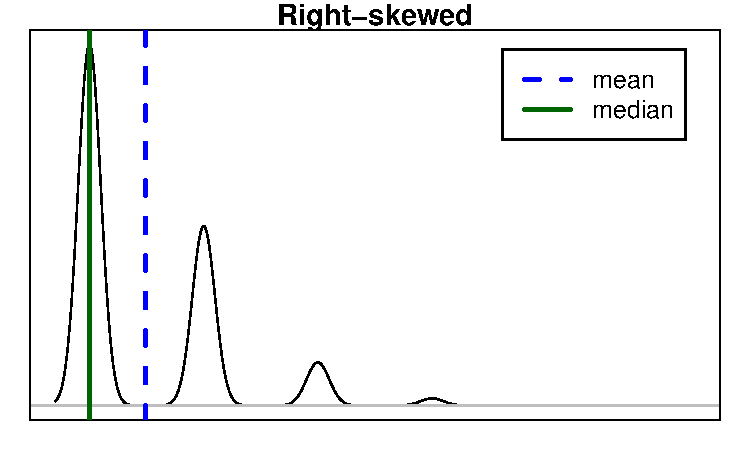
\includegraphics[width=0.33\textwidth]{1-6_numerical_data/figures/mean_med/rs}
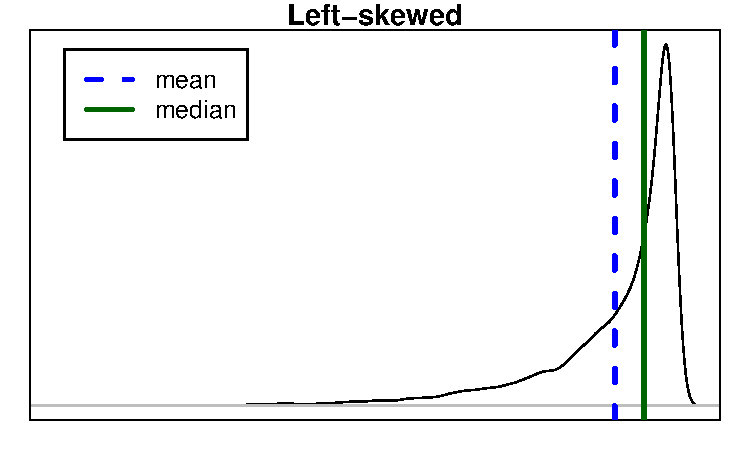
\includegraphics[width=0.33\textwidth]{1-6_numerical_data/figures/mean_med/ls}\\
\end{center}

\end{frame}

%%%%%%%%%%%%%%%%%%%%%%%%%%%%%%%%%%%%%

\begin{frame}
\frametitle{Practice}

\pq{{\small Which is most likely true for the distribution of percentage of time actually spent taking notes in class versus on Facebook, Twitter, etc.?}}

\vspace{-0.5cm}

\begin{columns}
\column{0.7\textwidth}
\begin{center}
\includegraphics[width=0.9\textwidth]{1-6_numerical_data/figures/notes_perc/notes_perc_hist}
\end{center}
\column{0.3\textwidth}
$\:$ \\
$\:$ \\
\soln{\only<2>{\red{median: 80\% \\ mean: 76\%}}}
\end{columns}

{\small
\begin{multicols}{2}
\begin{enumerate}[(a)]
\item mean$>$ median
\solnMult{mean $<$ median}
\item mean $\approx$ median
\item impossible to tell
\end{enumerate}
\end{multicols}
}

\end{frame}

%%%%%%%%%%%%%%%%%%%%%%%%%%%%%%%%%%%%%

\subsection{Transforming data}

%%%%%%%%%%%%%%%%%%%%%%%%%%%%%%%%%%%%

\begin{frame}
\frametitle{Extremely skewed data}

When data are extremely skewed, transforming them might make modeling easier. A common transformation is the \hl{log transformation}.

$\:$ \\
\pause
The histograms on the left shows the distribution of number of basketball games attended by students. The histogram on the right shows the distribution of log of number of games attended.

\begin{center}
\includegraphics[width=0.5\textwidth]{1-6_numerical_data/figures/basket_games/basket_games_hist}
\includegraphics[width=0.5\textwidth]{1-6_numerical_data/figures/basket_games/basket_games_hist_log}
\end{center}

\end{frame}

%%%%%%%%%%%%%%%%%%%%%%%%%%%%%%%%%%%%

\begin{frame}
\frametitle{Pros and cons of transformations}

\begin{itemize}

\item Skewed data are easier to model with when they are transformed because outliers tend to become far less prominent after an appropriate transformation. \\
$\:$ \\
\renewcommand{\arraystretch}{1.5}
\begin{tabular}{l r r r r }
\# of games		&  70 	& 50 		& 25 		 		& $\cdots$ \\
log(\# of games)	& 4.25	& 3.91 	& 3.22 	 	& $\cdots$
\end{tabular}

$\:$ \\

\item However, results of an analysis might be difficult to interpret because the log of a measured variable is usually meaningless.

\end{itemize}

\pause

\dq{What other variables would you expect to be extremely skewed?}

\soln{\pause{Salary, housing prices, etc.}}

\end{frame}

%%%%%%%%%%%%%%%%%%%%%%%%%%%%%%%%%%%%

\subsection{Mapping data}

%%%%%%%%%%%%%%%%%%%%%%%%%%%%%%%%%%%%

\begin{frame}
\frametitle{Intensity maps}

\dq{What patterns are apparent in the change in population between 2000 and 2010?}

\begin{center}
\includegraphics[width=0.95\textwidth]{1-6_numerical_data/figures/change_in_pop_intensity}
\end{center}

\ct{\webURL{http://projects.nytimes.com/census/2010/map}}

\end{frame}


%%%%%%%%%%%%%%%%%%%%%%%%%%%%%%%%%%%%
%%%%%%%%%%%%%%%%%%%%%%%%%%%%%%%%%%%%

\section{Considering categorical data}

%%%%%%%%%%%%%%%%%%%%%%%%%%%%%%%%%%%%

\subsection{Contingency tables and bar plots}

%%%%%%%%%%%%%%%%%%%%%%%%%%%%%%%%%%%%

\begin{frame}
\frametitle{Contingency tables}

A table that summarizes data for two categorical variables is called a \hl{contingency table}.

$\:$ \\
\pause
The contingency table below shows the distribution of students' genders and whether or not they are looking for a spouse while in college.

\begin{center}
\begin{tabular}{l l cc rr}
					& 			& \multicolumn{2}{c}{{looking for spouse}} \\
  \cline{3-4}
					&			& No	& Yes	& Total & \hspace{3mm}  \\ 
  \cline{2-5}
\multirow{2}{*}{{gender}}& Female 		& 86 	& 51 		& 137 \\ 
  					& Male 		& 52 	& 18	 	& 70\\ 
  \cline{2-5}
  					& Total		& 138& 69	&  207 \\
  \cline{2-5}
\end{tabular}
\end{center}

\end{frame}

%%%%%%%%%%%%%%%%%%%%%%%%%%%%%%%%%%%%

\begin{frame}
\frametitle{Bar plots}

A \hl{bar plot} is a common way to display a single categorical variable. A bar plot where proportions instead of frequencies are shown is called a \hl{relative frequency bar plot}.

\begin{center}
\includegraphics[width=0.45\textwidth]{1-7_categorical_data/figures/gender_spouse/gender_bar}
\includegraphics[width=0.45\textwidth]{1-7_categorical_data/figures/gender_spouse/gender_rel_bar}
\end{center}

\pause

\dq{How are bar plots different than histograms?}

\soln{\pause{{\scriptsize Bar plots are used for displaying distributions of categorical variables, while histograms are used for numerical variables. The x-axis in a histogram is a number line,  hence the order of the bars cannot be changed, while in a bar plot the categories can be listed in any order (though some orderings make more sense than others, especially for ordinal variables.)}}}

\end{frame}

%%%%%%%%%%%%%%%%%%%%%%%%%%%%%%%%%%

%%%%%%%%%%%%%%%%%%%%%%%%%%%%%%%%%%%%

\subsection{Row and column proportions}

%%%%%%%%%%%%%%%%%%%%%%%%%%%%%%%%%%%%

\begin{frame}
\frametitle{Choosing the appropriate proportion}

\dq{Does there appear to be a relationship between gender and whether the student is looking for a spouse in college?}

\begin{center}
\begin{tabular}{l l cc r}
					& 			& \multicolumn{2}{c}{{looking for spouse}} \\
  \cline{3-4}
					&			& No	& Yes	& Total \\ 
  \cline{2-5}
\multirow{2}{*}{{gender}}& Female 		& 86 	& 51 		& 137 \\ 
  					& Male 		& 52 	& 18	 	& 70\\ 
  \cline{2-5}
  					& Total		& 138& 69	&  207 \\
  \cline{2-5}
\end{tabular}
\end{center}

\pause

To answer this question we examine the row proportions: 

\pause

\begin{itemize}

\item \% Females looking for a spouse: $51 / 137 \approx 0.37$ \\

\pause

\item \% Males looking for a spouse: $18 / 70 \approx 0.26$ \\

\end{itemize}

\end{frame}

%%%%%%%%%%%%%%%%%%%%%%%%%%%%%%%%%%%%

\subsection{Segmented bar and mosaic plots}

%%%%%%%%%%%%%%%%%%%%%%%%%%%%%%%%%%%%

\begin{frame}
\frametitle{Segmented bar and mosaic plots}

\dq{What are the differences between the three visualizations shown below?}

\begin{center}
\includegraphics[width=0.33\textwidth]{1-7_categorical_data/figures/gender_spouse/gender_seg_bar}
\includegraphics[width=0.33\textwidth]{1-7_categorical_data/figures/gender_spouse/gender_rel_seg_bar}
\includegraphics[width=0.33\textwidth]{1-7_categorical_data/figures/gender_spouse/gender_mosaic}
\end{center}

\end{frame}

%%%%%%%%%%%%%%%%%%%%%%%%%%%%%%%%%%%%

\subsection{Pie charts}

%%%%%%%%%%%%%%%%%%%%%%%%%%%%%%%%%%%%

\begin{frame}
\frametitle{Pie charts}

\dq{Can you tell which order encompasses the lowest percentage of mammal species?}

\vspace{-0.5cm}

\begin{center}
\includegraphics[width=0.4\textwidth]{1-7_categorical_data/figures/mammal_pie_chart/mammal_pie_chart}
\includegraphics[width=0.2\textwidth]{1-7_categorical_data/figures/mammal_pie_chart/mammal_pie_chart_legend}
\end{center}

\ct{Data from \webURL{http://www.bucknell.edu/msw3}.}

\end{frame}


%%%%%%%%%%%%%%%%%%%%%%%%%%%%%%%%%%%%

\subsection{Comparing numerical data across groups}

%%%%%%%%%%%%%%%%%%%%%%%%%%%%%%%%%%%%

\begin{frame}
\frametitle{Side-by-side box plots}

\dq{Does there appear to be a relationship between class year and number of clubs students are in?}

\begin{center}
\includegraphics[width=\textwidth]{1-7_categorical_data/figures/year_clubs/year_clubs}
\end{center}

\end{frame}

%%%%%%%%%%%%%%%%%%%%%%%%%%%%%%%%%%%%


%%%%%%%%%%%%%%%%%%%%%%%%%%%%%%%%%%%%

\section{Case study: Gender discrimination}

%%%%%%%%%%%%%%%%%%%%%%%%%%%%%%%%%%%%

\subsection{Study description and data}

%%%%%%%%%%%%%%%%%%%%%%%%%%%%%%%%%%%%

\begin{frame}
\frametitle{Gender discrimination}

\begin{itemize}

\item In 1972, as a part of a study on gender discrimination, 48 male bank supervisors were each given the same personnel file and asked to judge whether the person should be promoted to a branch manager job that was described as ``routine". 

\item The files were identical except that half of the supervisors had files showing the person was male while the other half had files showing the person was female.

\item It was randomly determined which supervisors got ``male" applications and which got ``female" applications.  

\item Of the 48 files reviewed, 35 were promoted. 

\item The study is testing whether females are unfairly discriminated against.  
\end{itemize}

\dq{Is this an observational study or an experiment?} \soln{\onslide<2->{Experiment}}

\ct{B.Rosen and T. Jerdee (1974), ``Influence of sex role stereotypes on personnel decisions", J.Applied Psychology, 59:9-14.}

\end{frame}


%%%%%%%%%%%%%%%%%%%%%%%%%%%%%%%%%%%%

\begin{frame}
\frametitle{Data}

\dq{At a first glance, does there appear to be a relatonship between promotion and gender?}

\begin{center}
\begin{tabular}{ll  cc c} 
  		&				& \multicolumn{2}{c}{\textit{Promotion}} \\
\cline{3-4}
							&			& Promoted	& Not Promoted 	& Total	\\
\cline{2-5}
\multirow{2}{*}{\textit{Gender	}}	&Male 		& 21	 	& 3		& 24 	\\
							&Female		& 14	 	& 10 	 	& 24 \\
\cline{2-5}
							&Total		& 35		& 13		& 48 \\
\end{tabular}
\end{center}

\pause

\textbf{\% of males promoted: $21 / 24 = 0.875$} \\
\textbf{\% of females promoted: $14 / 24 = 0.583$}

\end{frame}

%%%%%%%%%%%%%%%%%%%%%%%%%%%%%%%%%%%%

\begin{frame}
\frametitle{Practice}

\pq{We saw a difference of almost 30\% (29.2\% to be exact) between the proportion of male and female files that are promoted. Based on this information, which of the below is true?}

\begin{enumerate}[(a)]

\item If we were to repeat the experiment we will definitely see that more female files get promoted. This was a fluke.

\item Promotion is dependent on gender, males are more likely to be promoted, and hence there is gender discrimination against women in promotion decisions. \soln{\only<2>{\red{Maybe}}}

\item The difference in the proportions of promoted male and female files is due to chance, this is not evidence of gender discrimination against women in promotion decisions. \soln{\only<2>{\red{Maybe}}}

\item Women are less qualified than men, and this is why fewer females get promoted.

\end{enumerate}

\end{frame}

%%%%%%%%%%%%%%%%%%%%%%%%%%%%%%%%%%%%

\subsection{Competing claims}

%%%%%%%%%%%%%%%%%%%%%%%%%%%%%%%%%%%%%

\begin{frame}
\frametitle{Two competing claims}

\begin{enumerate}

\item ``There is nothing going on." \\
Promotion and gender are \hl{independent}, no gender discrimination, observed difference in proportions is simply due to chance. $\rightarrow$ \hl{Null hypothesis}

\pause

\item ``There is something going on." \\
Promotion and gender are \hl{dependent}, there is gender discrimination, observed difference in proportions is not due to chance. $\rightarrow$ \hl{Alternative hypothesis}

\end{enumerate}

\end{frame}

%%%%%%%%%%%%%%%%%%%%%%%%%%%%%%%%%%%%

\begin{frame}
\frametitle{A trial as a hypothesis test}

\twocol{0.5}{0.5}
{
\begin{itemize}

\item Hypothesis testing is very much like a court trial.

\item $H_0$: Defendant is innocent \\
$H_A$: Defendant is guilty

\item We then present the evidence - collect data.

\end{itemize}
}
{
\includegraphics[width=\textwidth]{1-8_gender_discrimination/figures/trial}
}

\begin{itemize}

\item Then we judge the evidence - ``Could these data plausibly have happened by chance if the null hypothesis were true?"
\begin{itemize}
\item If they were very unlikely to have occurred, then the evidence raises more than a reasonable doubt in our minds about the null hypothesis.
\end{itemize}

\item Ultimately we must make a decision. How unlikely is unlikely?

\end{itemize}

\ct{Image from \webURL{http://www.nwherald.com/_internal/cimg!0/oo1il4sf8zzaqbboq25oevvbg99wpot}.}

\end{frame}

%%%%%%%%%%%%%%%%%%%%%%%%%%%%%%%%%%%%%

\begin{frame}
\frametitle{A trial as a hypothesis test (cont.)}

\begin{itemize}

\item If the evidence is not strong enough to reject the assumption of innocence, the jury returns with a verdict of ``not guilty".
\begin{itemize}
\item The jury does not say that the defendant is innocent, just that there is not enough evidence to convict.
\item The defendant may, in fact, be innocent, but the jury has no way of being sure.
\end{itemize}

\item Said statistically, we fail to reject the null hypothesis.
\begin{itemize}
\item We never declare the null hypothesis to be true, because we simply do not know whether it's true or not.
\item Therefore we never ``accept the null hypothesis".
\end{itemize}

\end{itemize}

\end{frame}

%%%%%%%%%%%%%%%%%%%%%%%%%%%%%%%%%%%%%

\begin{frame}
\frametitle{A trial as a hypothesis test (cont.)}

\begin{itemize}

\item In a trial, the burden of proof is on the prosecution.

\item In a hypothesis test, the burden of proof is on the unusual claim.

\item The null hypothesis is the ordinary state of affairs (the status quo), so it's the alternative hypothesis that we consider unusual and for which we must gather evidence.

\end{itemize}

\end{frame}

%%%%%%%%%%%%%%%%%%%%%%%%%%%%%%%%%%%%%

\begin{frame}
\frametitle{Recap: hypothesis testing framework}

\begin{itemize}
\item We start with a \hl{null hypothesis ($H_0$)} that represents the status quo.
\item We also have an \hl{alternative hypothesis ($H_A$)} that represents our research question, i.e. what we're testing for.
\item We conduct a hypothesis test under the assumption that the null hypothesis is true, either via simulation (today) or theoretical methods (later in the course).
\item If the test results suggest that the data do not provide convincing evidence for the alternative hypothesis, we stick with the null hypothesis. If they do, then we reject the null hypothesis in favor of the alternative.
\end{itemize}

\end{frame}

%%%%%%%%%%%%%%%%%%%%%%%%%%%%%%%%%%%%

\subsection{Testing via simulation}

%%%%%%%%%%%%%%%%%%%%%%%%%%%%%%%%%%%%%

\begin{frame}
\frametitle{Simulating the experiment...}

... under the assumption of independence, i.e. leave things up to chance. \\

\vspace{0.5cm}

If results from the simulations based on the \hl{chance model} look like the data, then we can determine that the difference between the proportions of promoted files between males and females was simply \hl{due to chance} (promotion and gender are independent). \\

\vspace{0.5cm}

If the results from the simulations based on the chance model do not look like the data, then we can determine that the difference between the proportions of promoted files between males and females was not due to chance, but \hl{due to an actual effect of gender} (promotion and gender are dependent).

\end{frame}

%%%%%%%%%%%%%%%%%%%%%%%%%%%%%%%%%%%%

\begin{frame}
\frametitle{Application activity: simulating the experiment}

\app{
Use a deck of playing cards to simulate this experiment.

\begin{enumerate}
\item Let a face card represent \textit{not promoted} and a non-face card represent a \textit{promoted}. Consider aces as face cards.
\begin{itemize}
\item Set aside the jokers.
\item Take out 3 aces $\rightarrow$ there are exactly 13 face cards left in the deck (face cards: A, K, Q, J).
\item Take out a number card $\rightarrow$ there are exactly 35 number (non-face) cards left in the deck (number cards: 2-10).
\end{itemize}
\item Shuffle the cards and deal them intro two groups of size 24, representing males and females. 
\item Count and record how many files in each group are promoted (number cards).

\item Calculate the proportion of promoted files in each group and take the difference (male - female), and record this value.

\item Repeat steps 2 - 4 many times.

\end{enumerate}
}

\end{frame}

%%%%%%%%%%%%%%%%%%%%%%%%%%%%%%%%%%%%

\begin{frame}
\frametitle{Step 1}

\begin{center}
\includegraphics[width=\textwidth]{1-8_gender_discrimination/figures/step1}
\end{center}

\end{frame}


%%%%%%%%%%%%%%%%%%%%%%%%%%%%%%%%%%%%

\begin{frame}
\frametitle{Step 2 - 4}

\begin{center}
\includegraphics[width=\textwidth]{1-8_gender_discrimination/figures/step2}
\end{center}

\end{frame}


%%%%%%%%%%%%%%%%%%%%%%%%%%%%%%%%%%%%

\subsection{Checking for independence}

%%%%%%%%%%%%%%%%%%%%%%%%%%%%%%%%%%%%

\begin{frame}
\frametitle{Practice}

\pq{Do the results of the simulation you just ran provide convincing evidence of gender discrimination against women, i.e. dependence between gender and promotion decisions?}

\begin{enumerate}[(a)]
\item No, the data do not provide convincing evidence for the alternative hypothesis, therefore we can't reject the null hypothesis of independence between gender and promotion decisions. The observed difference between the two proportions was due to chance.
\solnMult{Yes, the data provide convincing evidence for the alternative hypothesis of gender discrimination against women in promotion decisions. The observed difference between the two proportions was due to a real effect of gender.}
\end{enumerate}

\end{frame}

%%%%%%%%%%%%%%%%%%%%%%%%%%%%%%%%%%%%

\begin{frame}
\frametitle{Simulations using software}

These simulations are tedious and slow to run using the method described earlier. In reality, we use software to generate the simulations. The dot plot below shows the distribution of simulated differences in promotion rates based on 100 simulations.

\begin{center}
\includegraphics[width=0.8\textwidth]{1-8_gender_discrimination/figures/discRandDotPlot/discRandDotPlot}
\end{center}

\end{frame}

%%%%%%%%%%%%%%%%%%%%%%%%%%%%%%%%%%%%%

%%%%%%%%%%%%%%%%%%%%%%%%%%%%%%%%%%%%

\end{document}